\documentclass[12pt, a4paper, twoside]{report}

% --- Language and Fonts ---
\usepackage[utf8]{inputenc}
\usepackage[T1]{fontenc}
\usepackage{times}
\usepackage[english, polish]{babel}

% --- Page Layout ---
\usepackage[a4paper, 
    top=2.5cm, bottom=2.5cm, 
    left=3.0cm,
    right=2.5cm, 
    headsep=1.2cm]{geometry}

\usepackage{setspace}
\singlespacing

\usepackage{indentfirst}
\setlength{\parindent}{0.7cm}

\usepackage{graphicx}
\usepackage{float}

% --- Bibliography Setup ---
\usepackage[style=numeric, sorting=none, backend=biber, doi=true, isbn=false, natbib=true]{biblatex}
\addbibresource{intro_references.bib}

\DeclareFieldFormat{doi}{%
  \newline \url{https://doi.org/#1}}

\usepackage{hyperref}
\hypersetup{
    colorlinks=true,
    linkcolor=blue,
    urlcolor=blue,
    citecolor=black
}

% --- Titles Formatting ---
\usepackage{titlesec}
\titleformat{\chapter}{\normalfont\fontsize{14}{16}\bfseries}{\thechapter.}{0.5em}{}
\titleformat{\section}{\normalfont\fontsize{13}{15}\bfseries}{\thesection.}{0.5em}{}
\titleformat{\subsection}{\normalfont\fontsize{12}{14}\bfseries}{\thesubsection.}{0.5em}{}
\titlespacing*{\chapter}{0pt}{0pt}{20pt}

% --- Captions and Tables ---
\usepackage{caption}
\DeclareCaptionFont{tenpt}{\fontsize{10}{12}\selectfont}
\captionsetup{font=tenpt, labelfont=tenpt, justification=centering}
\captionsetup[table]{skip=10pt}
\captionsetup[figure]{aboveskip=10pt, belowskip=10pt}

% --- Equations and Tables ---
\usepackage{amsmath}
\numberwithin{equation}{chapter}
\usepackage{booktabs}
\usepackage{longtable}
\usepackage{array}
\usepackage{multirow}
\usepackage{tabularx}

% -----------------------------------------------------------------
\begin{document}
\selectlanguage{english}

% --- TITLE PAGE ---
\begin{titlepage}
    \centering
    {\fontsize{16}{18}\selectfont \textbf{Wroc\l{}aw University of Science and Technology} \\}
    {\fontsize{14}{16}\selectfont Faculty of Information and Communication Technology \\}
    \rule{\textwidth}{1pt}

    \vspace{3cm}
    {\fontsize{20}{24}\selectfont MASTER THESIS \par}

    \vspace{2cm}
    {\fontsize{16}{18}\selectfont \textbf{Watermarking of Images Generated by Large Generative Models:\\[4pt]
    A Comparative Study of Imperceptible Marking Algorithms} \par}

    \vspace{1.5cm}
    {\fontsize{14}{16}\selectfont [Author Name] \par}

    \vspace{2cm}
    \begin{center}
        Supervisor \\
        Supervisor Name
    \end{center}

    \vfill
    \begin{flushleft}
    Keywords: digital watermarking, generative AI, latent diffusion models, image authentication, steganography, perceptual robustness
    \end{flushleft}
    \rule{\textwidth}{1pt}
    WROC\L{}AW 2026
\end{titlepage}

% --- ABSTRACTS ---
\pagenumbering{roman}

\chapter*{Abstract}

The rapid proliferation of AI-generated imagery---driven primarily by latent diffusion architectures such as Stable Diffusion, DALL-E, and Midjourney---has created a pressing need for reliable mechanisms of content provenance. This thesis investigates imperceptible digital watermarking as a technical response to that problem. I conduct a systematic literature survey and comparative evaluation of thirty-one watermarking algorithms, spanning classical frequency-domain transforms (DWT, DCT, SVD and their hybrids), deep learning encoder-decoder frameworks (HiDDeN, RivaGAN, StegaStamp), latent-space methods, and techniques designed to integrate watermarking directly into the diffusion generation process (Tree-Ring, The Stable Signature, Gaussian Shading, PTW, ZoDiac, and others). Selected algorithms are implemented across multiple generative AI environments and evaluated on a unified benchmark covering imperceptibility metrics (PSNR, SSIM), robustness to a defined suite of image attacks (JPEG compression, geometric transforms, noise, regeneration), and detection reliability (bit accuracy, AUC). I find that pipeline-integrated methods---those embedding the watermark during generation rather than post-hoc---offer substantially higher robustness against regeneration attacks, at the cost of requiring control over the generation model itself. Classical transform methods remain competitive in low-attack scenarios but degrade rapidly under modern compression pipelines. No single method dominates all evaluation axes simultaneously. The thesis concludes with a structured taxonomy of the methods, a practical recommendation framework, and identified directions for future research.


\chapter*{Acknowledgements}

[To be completed.]

% --- LISTS ---
\tableofcontents
\listoffigures
\listoftables

% --- MAIN CONTENT ---
\clearpage
\pagenumbering{arabic}

%%%%%%%%%%%%%%%%%%%%%%%%%%%%%%%%%%%%%%%%%%%%%%%%%%%%%%%%%%%%%%%%%%
\chapter{Introduction}
%%%%%%%%%%%%%%%%%%%%%%%%%%%%%%%%%%%%%%%%%%%%%%%%%%%%%%%%%%%%%%%%%%

\section{Background and Motivation}
Something changed in 2022, and it changed fast. Stable Diffusion 1.4 was released publicly in August of that year \citep{rombach2022ldm}. DALL-E 2 had arrived a few months earlier, in April \citep{ramesh2022dalle2}. Midjourney v3, which was already producing results that confused professional photographers in online blind tests, launched that same summer \citep{holz2022midjourney}. Within eighteen months of those releases, high-quality generative image tools were running locally on consumer hardware. The images stopped looking artificial. They started looking real: not approximately real, but perceptually indistinguishable from photographs in controlled studies \citep{nightingale2022faces}.
\begin{figure}[H]
    \centering
    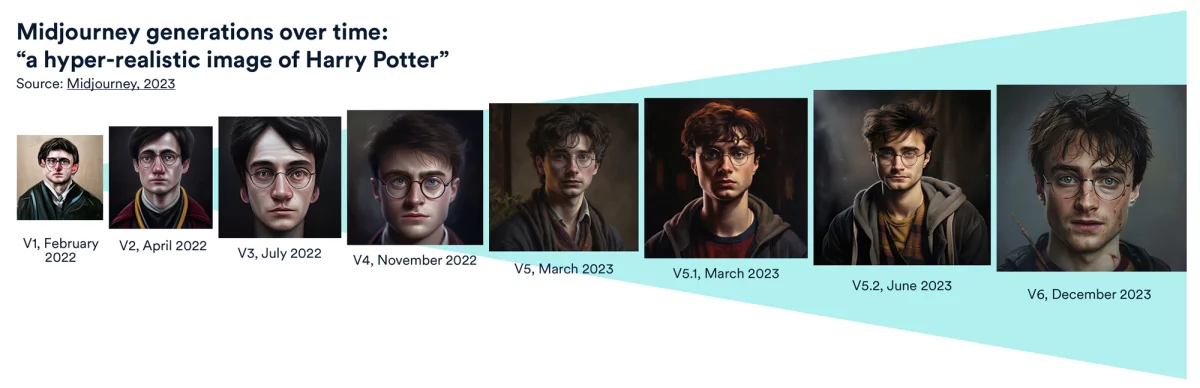
\includegraphics[width=0.8\textwidth]{download.png}
    \caption{AI generation improvement (illustrative example)~\citep{aiindex2024newatlas}.}
    \label{fig:ai-generation-improvement}
\end{figure}
The problem is not the images themselves. The problem is that they carry no intrinsic trace of their origin. A photograph taken with a Nikon D850 embeds EXIF metadata automatically: camera model, GPS coordinates, timestamp, lens, focal length and that can be used to identify the origin of the images and the validity of the owner \citep{exif2019spec}. Yes, That metadata can be stripped, but its absence is itself a signal. AI-generated images have no equivalent. A synthetically produced portrait inserted into a news article is, at the pixel level, identical to a real photograph. No forensic tool can recover what was never there to begin with, and the scale at which these images are being produced, billions per month across the major platforms by 2024 \citep{scale_citation}, makes manual review impossible.
 
Watermarking is the attempt to put something back. The term comes from papermaking, where semi-transparent patterns were pressed into the pulp during manufacture to indicate provenance and deter counterfeiting \citep{hunter1957papermaking}. Digital watermarking has existed as a formal research area since at least the early 1990s, with \citet{cox1997}'s 1997 paper on secure spread-spectrum watermarking establishing much of the vocabulary still in use. What has changed, radically, is the context: the threat model, the scale, and the capabilities of both the embedding side and the attack side \citep{cox2007book}.
 
The EU AI Act, adopted in March 2024, includes provisions requiring that AI-generated content be marked as such \citep{euaiact2024}. The US Executive Order on AI, signed in October 2023, directed federal agencies to develop standards for watermarking AI content \citep{biden2023eo}. NIST published preliminary guidelines in early 2024 \citep{nist2024synthetic}. The policy momentum is clear. The technical capability to fulfil those policies is, I will argue, still catching up.
 
This thesis is about that gap.

\section{Problem Statement}

Existing watermarking methods for AI-generated images are evaluated in isolation, each benchmarked against attack suites and distortion parameters selected by the authors to reflect the method's own design assumptions. There is no shared evaluation framework, and cross-method comparisons in the literature are therefore not directly commensurable. It is currently unclear which methods generalise beyond the conditions they were optimised for.
 
A secondary gap is architectural. No prior work has applied a mixture-of-experts formulation to the watermarking problem, despite the intuition that different transformation attacks call for different embedding strategies. Whether a learned routing over specialised sub-networks can improve robustness across a heterogeneous attack distribution remains an open question.
 
This thesis addresses both gaps.


\section{Research Objectives and Questions}
 
This thesis pursues two primary objectives. The first is to evaluate existing watermarking methods for AI-generated images under a unified, consistent framework, in order to establish which methods generalise beyond the conditions they were designed for. The second is to investigate whether a mixture-of-experts architecture, not previously applied to image watermarking, can improve robustness across a heterogeneous set of transformation attacks.
 
These objectives give rise to the following research questions:
 
\begin{enumerate}
    \item To what extent do published watermarking methods maintain detection performance when evaluated outside their own benchmarking conditions, under a fixed and uniform attack protocol?
    \item How do existing methods compare in terms of the robustness-imperceptibility trade-off when assessed on a shared image corpus with consistent distortion parameters?
    \item Can a mixture-of-experts formulation, in which specialised sub-networks handle distinct transformation regimes, achieve higher robustness across a heterogeneous attack distribution than single-architecture baselines?
    \item What are the computational cost implications of a mixture-of-experts watermarking model relative to existing approaches, and does the architecture remain viable at generation scale?
\end{enumerate}
 

\section{Scope and Limitations}

This thesis focuses exclusively on still images generated by large generative models, specifically latent diffusion models. Video watermarking is a related but distinct problem, and including it would roughly double the scope of the work. Text and audio watermarking are outside scope entirely, though both are active research areas with some methodological overlap.
The comparative evaluation is restricted to the twenty algorithms catalogued in Chapter~2, chosen to represent all major technical families while remaining tractable to implement and evaluate within a single thesis. This is not exhaustive. Relevant papers published after the literature cutoff of [date to be confirmed] are not included; I note where awareness of subsequent work would likely change my conclusions.
The evaluation benchmark uses a fixed image resolution of [resolution], a defined attack suite based on the WAVES protocol, and 500 images drawn from [dataset]. This constraint is imposed by the computational demands of the evaluation pipeline: running the full attack suite, decoding metrics, and MoE architecture training across twenty methods at full capacity renders a larger image set intractable within the available compute budget. Real-world deployment is more varied and more hostile than any controlled benchmark captures. The reported numbers are indicators, not deployment guarantees.

\section{Thesis Contribution}

The primary contributions of this thesis are as follows. First, a structured taxonomy of current AI image watermarking approaches organised along two interpretively useful axes. Second, a unified Python evaluation harness that allows direct comparison across methods with otherwise incompatible evaluation settings. Third, empirical results across all implemented algorithms on a common benchmark, using the WAVES protocol as the shared evaluation standard, providing the first systematic cross-method comparison under consistent attack conditions and distortion parameters. Fourth, identification of methodological inconsistencies in the existing literature that complicate interpretation of prior results. Fifth, a novel mixture-of-experts watermarking architecture, in which specialised sub-networks are trained to embed and detect watermarks under distinct transformation regimes, with a learned gating mechanism routing each image to the appropriate expert at inference time; to the author's knowledge, this is the first application of a mixture-of-experts formulation to the image watermarking problem. Sixth, a practical recommendation framework for practitioners.

\section{Thesis Structure}

Chapter~2 reviews the literature in order of technical generation, beginning with classical frequency-domain methods and ending with the most recent diffusion-native approaches. Chapter~3 describes the dataset, implementation environment, and evaluation design. Chapter~4 presents experimental results. Chapter~5 discusses what those results mean and---equally important---where they fall short. Chapter~6 concludes with practical recommendations and directions for future work.

\section{State of the Art Summary}

The field divides naturally into three technical generations, though the boundaries between them are messier in practice than any taxonomy suggests.

The first generation, dominant through the early 2000s, embedded watermarks by modifying coefficients in frequency-domain transform spaces---DCT, DWT, SVD, and combinations thereof. Cox et al.~\cite{cox1997} is the canonical early reference. These methods are computationally cheap, mathematically well-understood, and reasonable at hiding signals in images that will be stored and transmitted without significant modification. Against JPEG-Q50 compression or even moderate geometric transforms, most of them fail. They were designed for a different world.

The second generation arrived with deep learning. HiDDeN~\cite{zhu2018hidden}, published by Zhu et al.\ at NeurIPS 2018, introduced the encoder-noise-decoder training paradigm that most subsequent deep watermarking methods follow. RivaGAN~\cite{[rivagan]}, StegaStamp~\cite{tancik2020stegastamp}, and the self-supervised latent space method~\cite{[ssl_wm]} represent the maturation of this approach. These methods learn to exploit natural image statistics in ways that transform methods cannot, and they handle compression and noise much better. Their Achilles heel, it turns out, is the regeneration attack---passing a watermarked image through a second generative model to produce a clean, unwatermarked version.

The third generation integrates watermarking into the generative process itself. Tree-Ring~\cite{[treering]}, proposed by Wen et al.\ in 2023, modifies the initial noise vector of the diffusion process in a way that survives denoising. The Stable Signature~\cite{[stablesig]}, from Fernandez et al.\ also in 2023, fine-tunes the VAE decoder of a latent diffusion model to consistently output watermarked images. Gaussian Shading~\cite{[gaussshading]}, PTW~\cite{[ptw]}, ZoDiac~\cite{[zodiac]}, and a cluster of very recent methods extend this direction. These approaches are qualitatively different because they do not add a watermark to an image---they make the watermark part of what generation \textit{means} for that model.

%%%%%%%%%%%%%%%%%%%%%%%%%%%%%%%%%%%%%%%%%%%%%%%%%%%%%%%%%%%%%%%%%%
\chapter{Literature Review}
%%%%%%%%%%%%%%%%%%%%%%%%%%%%%%%%%%%%%%%%%%%%%%%%%%%%%%%%%%%%%%%%%%
\subsection{Deep Learning and Diffusion-Era Watermarking}

\subsubsection{Framing: Evaluation Infrastructure, Cryptographic Security, and the Regeneration Threat}

Before surveying individual methods, I need to establish the evaluative vocabulary the field has converged on. Every claim of ``robustness'' or ``imperceptibility'' is only meaningful relative to the metrics, attack protocols, and security definitions against which it's measured. This sounds like housekeeping. It isn't. Conflating performance on one axis with overall capability has been one of the most persistent problems in the watermarking literature, and I'll be honest that I'll be doing it too in places where the data forces my hand.

Three distinct frameworks govern evaluation: image quality, attack benchmarking, and cryptographic security.

On image quality: the two foundational perceptual metrics are Peak Signal-to-Noise Ratio (PSNR) and the Structural Similarity Index Measure (SSIM). PSNR expresses the ratio between maximum possible pixel energy and the distortion energy introduced by watermarking, in decibels --- values above 35~dB are conventionally considered imperceptible \citep{huynhthu2008}. SSIM, introduced by \citet{wang2004} in 2004, departed from pixel-error framing entirely. The intuition behind it still strikes me as genuinely elegant: human visual perception is adapted for extracting structural information from scenes, so a quality metric should measure degradation of structure rather than deviation of pixel values. SSIM does that by assessing luminance, contrast, and structure separately, with values above 0.98 indicating perceptually transparent embedding. For diffusion-era methods that operate at the distribution level rather than the pixel level, a third metric becomes necessary. Fr\'{e}chet Inception Distance, introduced by \citet{heusel2017} in 2017, captures whether embedding shifts the statistical distribution of images in ways invisible to pixel-level metrics but detectable in feature space, by computing the Fr\'{e}chet distance between multivariate Gaussian distributions fitted to Inception-v3 feature vectors. For classical methods this concern is irrelevant. For noise-injection approaches like Gaussian Shading, which explicitly target distribution-lossless embedding, it's central. Beyond these, robustness evaluations standardly report True Positive Rate at fixed False Positive Rate (TPR@FPR), Normalised Correlation (NC) for classical methods, and bit accuracy for multi-bit encoders. The choice of which metrics to report --- and crucially, at which attack strength --- determines what ``state of the art'' actually means. The benchmarking literature exploits this directly.

The attack taxonomy situation was a mess before 2024. Each paper evaluated robustness against its own hand-picked attack set, making cross-method comparisons unreliable in ways authors either didn't notice or chose not to flag. \citet{an2024} addressed this with WAVES --- Watermark Analysis Via Enhanced Stress-testing --- published at ICML 2024. WAVES integrates detection and identification tasks under a standardised evaluation protocol spanning traditional image distortions and advanced diffusive and adversarial attack variants, examining both quality degradation and watermark survival jointly. What makes WAVES significant is the treatment of regeneration. Prior work considered only single-pass regeneration. WAVES introduces rinsing regenerations: multiple cycles of noising and denoising through a pre-trained diffusion model, plus prompted and mixed variants. Even Tree-Ring, previously considered robust, doesn't survive these conditions. That finding landed harder than I expected when I first read it.

The regeneration attack itself was formalised theoretically by \citet{zhao2023}, who showed that invisible pixel-level watermarks are provably removable by generative AI. Their approach corrupts the image by adding Gaussian noise to its latent representation and reconstructing via a generative model, achieving over 99\% removal rates for DWT-DCT-SVD, RivaGAN, and SSL watermarking. The information-theoretic argument is clean and uncomfortable: the diffusion model's reconstruction marginalises over the degrees of freedom occupied by the watermark signal, because those degrees of freedom were not part of the semantic content used to condition the denoiser. The watermark lives in a subspace the model doesn't care about preserving. This renders the entire prior threat model --- JPEG compression, additive noise, geometric distortions --- insufficient, and it motivates every method I discuss below. WAVES defines the evaluation standard used in Chapter~4 of this thesis.

Cryptographic security is a dimension that perceptual and robustness metrics cannot capture at all. \citet{cox2007}'s 2007 textbook situates digital watermarking within the broader cryptographic communications framework, distinguishing between robustness attacks that seek to destroy the mark and protocol attacks that exploit the scheme's own structure --- including inversion attacks where an adversary uses a watermarked image to falsely claim ownership of an unwatermarked one. This is the root of the False Positive Problem in SVD-based classical methods: extraction depends on the U and V matrices of any decomposition rather than a secret key, providing no cryptographic binding. A formally secure watermark must satisfy completeness (every watermarked image is detected), soundness (an adversary without the key cannot forge a valid mark), and distortion-freeness (embedding doesn't shift the image distribution). These properties together constitute a cryptographic primitive in the strict sense --- an adversary without the key cannot produce a watermarked output that passes detection, even given polynomially many genuine watermarked examples as reference. Which methods satisfy these guarantees formally, rather than empirically, is a question I return to throughout. The honest answer is: fewer than the literature implies.

\subsubsection{Learned Encoder--Decoder Watermarking}

The earliest neural watermarking works preserved the structural assumption of classical methods --- modify the cover image after generation --- but replaced the fixed transform with a learned one, enabling joint optimisation of imperceptibility and robustness that no classical method could achieve. The design was right. The threat model turned out to be wrong, but that came later.

\citet{zhu2018} introduced HiDDeN: an encoder hides an $N$-bit message inside an image, a paired decoder recovers it, and an adversarial discriminator enforces perceptual fidelity, with a differentiable noise layer simulating JPEG, cropping, and Gaussian noise during training. Near-perfect bit accuracy under moderate compression at PSNR above 33~dB for a 30-bit payload. The encoder-decoder paradigm became the template for everything that followed, and it's worth sitting with why: the joint optimisation across imperceptibility, robustness, and capacity was simply not achievable with hand-crafted transforms. HiDDeN made the problem learnable.

\citet{ahmadi2019} extended this with ReDMark, using residual fully convolutional networks that diffuse the watermark signal across the full spatial extent of the image rather than concentrating it locally. Spatial diffusion makes the mark harder to localise and excise without damaging the whole image. What ReDMark also formalised explicitly is something that should have been obvious but wasn't always treated as such: the training-time attack distribution is itself a design choice. Train against JPEG and crop, get robustness against JPEG and crop. Nothing else is guaranteed. \citet{wen2019} pushed this further with ROMark, applying robust optimisation from adversarial machine learning to the training objective, minimising worst-case loss across multiple attack types rather than average-case loss and framing robustness as a minimax problem. This yields quantified rather than purely empirical guarantees. It's a conceptual step closer to the cryptographic security definitions above, though it doesn't reach them.

\citet{tancik2020} extended HiDDeN's architecture to the physical domain with StegaStamp, training with perspective warps, colour shifts, and moir\'{e} simulation to survive camera re-capture of printed outputs. Bit error rates below 0.01 from smartphone photographs at PSNR 31--34~dB. It's a genuinely different deployment context that most watermarking papers ignore, and the results still hold up. \citet{zhang2019} offered RivaGAN, using an attention mechanism to steer the encoder toward semantically salient image regions and a GAN adversarial loss in place of a fixed discriminator, yielding NC above 0.97 under cropping and affine transformations. RivaGAN's content-adaptive design anticipates a principle confirmed by subsequent steganalysis work: content-agnostic watermarks that embed a fixed pattern without adapting to image structure are susceptible to steganalysis-based removal, while content-adaptive methods demonstrate substantially higher resistance. I find that result satisfying in retrospect, though I'm not fully convinced the causal mechanism is entirely the content-adaptivity rather than the GAN training dynamics. The two are entangled in RivaGAN's design and the paper doesn't really disentangle them.

\citet{bui2023} demonstrated a qualitatively different design point with RoSteALS, decoupling payload embedding from the distribution of cover images entirely by operating in the latent space of a frozen pretrained autoencoder. A lightweight secret encoder of just 300k parameters, perfect secret recovery performance on three benchmarks. The frozen autoencoder already captures the natural image distribution; the secret encoder only modulates the latent code, inheriting the autoencoder's semantic robustness at a fraction of the training cost. \citet{fernandez2022} reframed the problem at the representation level with the SSL Watermark, embedding a watermark direction into the latent space of a frozen self-supervised DINO model via lightweight fine-tuning, detecting by checking whether a query image's embedding falls within the marked subspace. PSNR above 42~dB with AUC above 0.99 without per-image optimisation at inference time. The geometric view --- that the structure of learned representations is itself a carrier channel --- directly anticipated the diffusion-native methods that follow. I find this 2022 paper more prescient than it tends to get credit for.

InvisMark \citep{xu2024} represents the current ceiling of the post-hoc encoder-decoder paradigm: 256-bit payloads at PSNR around 51~dB with over 97\% bit accuracy across a comprehensive manipulation suite including high-resolution upscaling to 2K. Genuinely remarkable performance. And also, in a sense, peak performance on a paradigm with a structural flaw. The watermark is applied outside the generation graph, making it vulnerable to the semantic-level regeneration attacks formalised by \citet{zhao2023}. There's something instructive about that ceiling: optimising within a compromised paradigm will eventually get you somewhere, but it won't get you out.

Three things carry forward from this body of work: a neural encoder can hide more bits more robustly than any handcrafted transform; adversarial training over a realistic attack distribution is the correct approach to robustness; and the latent space of a pretrained model is itself a usable carrier channel. The shared weakness --- post-hoc watermarking outside the generation graph --- is precisely what the next generation of methods tried to solve.

\subsubsection{Diffusion-Native Watermarking}

The regeneration attack established a new design imperative. If superimposing a watermark on generated output means the watermark lives in degrees of freedom the generative model doesn't care about --- and therefore happily discards during reconstruction --- then the mark must be entangled with the generative process itself. The literature responds across four architectural strategies: fine-tuning model weights, injecting structure into the initial noise, using the diffusion trajectory as the embedding medium, and operating within the model's low-dimensional geometric subspaces. Each imposes different access requirements and offers a different security profile. None dominates the others.

\paragraph{Decoder fine-tuning and model-weight methods.}


The Stable Signature \citep{fernandez2023} pioneered weight embedding by fine-tuning the VAE decoder of a pre-trained latent diffusion model so that every image it decodes carries a fixed binary signature detectable by a paired extractor network. Because the watermark resides in decoder weights rather than image pixels, every output is inherently marked with no inference-time overhead --- bit accuracy above 0.99 on 48-bit payloads at PSNR above 38~dB. The fundamental weakness is susceptibility to adversarial decoder fine-tuning: an adversary who continues training the weights can drift them away from the marked state. PTW (Pivotal Tuning Watermarking, 2024) addresses this by anchoring the watermark to specific token embeddings through pivotal tuning, making the marked decoder state a stable fixed point that maintains bit accuracy above 0.96 after 500 steps of adversarial weight updates. The Flexible and Lightweight Framework \citep{xiong2023} demonstrates that the same fidelity and accuracy targets can be met with fewer than 1\% of the original decoder's parameters via low-rank adaptation, which matters enormously for any real deployment where per-user signature personalisation needs to be computationally viable at scale.

AquaLoRA \citep{feng2024} approaches weight embedding from a white-box protection angle, targeting the specific threat of checkpoint sharing on platforms like Civitai where malicious users can directly inspect and modify model weights. AquaLoRA merges watermark information into the U-Net of Stable Diffusion via a watermark LoRA module, with a scaling matrix enabling message updates without retraining. The two-stage design --- latent watermark pre-training followed by Prior Preserving Fine-Tuning --- ensures watermark learning doesn't degrade the model's generative distribution, while the LoRA integration means the mark is structurally fused with model weights rather than sitting in a separable module. WOUAF \citep{wouaf2024} pursues user attribution through weight modulation rather than decoder fine-tuning, binding the watermark to the specific user's generation context rather than the model checkpoint itself. Conceptually that's an important distinction: you're watermarking the use, not just the model.

\paragraph{Initial-noise injection.}
Tree-Ring Watermarks \citep{wen2023} embedded the mark in the initial noise vector by imposing a ring pattern in its Fourier domain, exploiting the near-determinism of DDIM sampling to make the pattern recoverable by diffusion inversion, requiring no model modification and reporting AUC above 0.99 under JPEG and brightness attacks at zero inference overhead. Then \citet{ci2024} performed a systematic re-examination --- RingID --- and found two overlooked phenomena that suggest Tree-Ring was underscrutinised when it first appeared. The distribution shift introduced by ring imprinting contributes substantially to robustness, but it cannot distinguish between different watermark keys. In a multi-user deployment, you can detect a watermark but not whose. RingID addresses this through a multi-channel heterogeneous framework, improving multi-key identification accuracy under rotation from near zero to 0.86.

Gaussian Shading \citep{yang2024} replaced the ring structure with something statistically principled: the watermark is mapped to a latent representation provably indistinguishable from the standard Gaussian prior, achieving distribution-lossless embedding by construction and eliminating FID degradation by design. Gaussian Shading++ \citep{yang2025} extended this with a double-channel design using pseudorandom error-correcting codes and ECDSA public-key signatures enabling third-party verification without sharing the secret key. That's a meaningful cryptographic advance that prior statistical approaches lacked. It also applies near-optimal soft-decision decoding treating the full generation and inversion pipeline as an AWGN channel --- a framing I find genuinely elegant --- substantially improving robustness under guidance-scale mismatch between embedding and detection time.

The PRC Watermark \citep{gunn2024} takes the most cryptographically rigorous position on noise-injection, selecting the initial noise using a pseudorandom error-correcting code derived from a secret key and providing formal soundness guarantees: an adversary without the key cannot construct a valid detection claim even with access to many watermarked images, formally eliminating the False Positive Problem at the theoretical level in a way that Tree-Ring and Gaussian Shading do not. I want to be careful here about what formal soundness actually buys in practice. It rules out key-free forgery attacks, but it doesn't automatically translate to robustness against every empirical attack in WAVES. The cryptographic and empirical threat models are not the same thing, and the watermarking literature sometimes lets formal results do more rhetorical work than they deserve.

CoSDA \citep{fang2025} identified a practical weakness shared by all inversion-based noise-injection methods --- inversion error --- and addressed it through two targeted mechanisms: compensation-based forward sampling to address condition mismatch between embedding and detection (prompt, guidance scale), and a drift-alignment approach where a neural network is trained adversarially to restore the original watermarked latent from the distorted counterpart. This work matters directly to this thesis because inversion error under guidance-scale mismatch represents a deployment gap affecting Tree-Ring, RingID, and original Gaussian Shading in real-world scenarios where generation and detection conditions are not identical. The gap between laboratory performance and deployment reality is something I found consistently underemphasised across this literature.

\paragraph{Low-dimensional subspace methods.}
Shallow Diffuse \citep{li2025} takes a geometrically motivated approach distinct from prior noise-injection methods. Rather than integrating watermarking throughout the entire diffusion sampling process, it decouples the steps by leveraging a low-dimensional subspace in the image generation process, ensuring a substantial portion of the watermark lies in the null space of this subspace and is effectively separated from image generation. The robustness argument is structurally different from anything in the noise-injection family: because the watermark occupies directions the diffusion model doesn't use for semantic generation, a regeneration pass that reconstructs semantic content leaves the watermark intact. That's a satisfying theoretical answer to the regeneration threat. Whether it holds against the rinsing attacks in WAVES is something I examine in Chapter~4.

\paragraph{Diffusion-trajectory and post-generation methods.}
ZoDiac \citep{wu2024} uses the diffusion model itself as the embedding medium, partially noising an existing image and denoising it with a watermark signal injected into the trajectory. AUC above 0.95 even under strong regeneration at PSNR above 37~dB --- a regime no pure encoder-decoder method achieves --- at the cost of a full denoising pass per image at embedding time. ROBIN \citep{huang2024} separates the embedding and concealment objectives explicitly: a robust watermark is implanted in an intermediate diffusion state and an adversarial optimisation over the prompt embedding guides the model to conceal the mark in the final output with minimal visible artefacts. The core move --- using the model's own generative capability as the concealment mechanism --- breaks the fundamental imperceptibility-robustness trade-off that constrains prior methods. DiffuseTrace \citep{diffusetrace2024} targets the partial-regeneration threat specifically, embedding a frequency-domain trace in the latent space that survives diffusion inpainting and SDEdit on unedited image regions, enabling forensic attribution of partially edited images. No prior method addressed that objective.

\paragraph{In-generation and latent-injection methods.}
LaWa \citep{lawa2024} bridges noise-injection and decoder fine-tuning by embedding the watermark directly within the generation trajectory, manipulating the latent representation during denoising rather than modifying the prior or the trained weights. Latent Watermark \citep{latentwm2024} proposes a plug-and-play latent-embedding scheme requiring no fine-tuning, making it deployable across different model checkpoints without retraining --- a practical advantage that fine-tuning approaches sacrifice. ProMark \citep{promark2024} advances causal attribution watermarking, embedding marks that encode the causal chain of generation decisions --- prompt, model configuration, sampling parameters --- enabling forensic reconstruction of the specific generation context rather than binary detection. GenPTW \citep{genptw2025} extends the in-generation paradigm to tamper localisation, embedding watermarks during generation in a way that enables both provenance tracing and spatial detection of which image regions have been subsequently altered.

\paragraph{Ownership, identity, and white-box protection.}
Several methods focus specifically on protecting model owner IP in scenarios where the adversary has direct weight access. PCDiff \citep{pcdiff2025} embeds ownership information during model training rather than at generation time, so the watermark is a structural property of the model's outputs and survives arbitrary downstream fine-tuning. TraceMark-LDM \citep{tracemark2025} handles the dual-use case where a model operator needs to prove both that an image came from their model and which specific licensed user generated it. A Watermark-Conditioned Diffusion Model for IP Protection \citep{wmcond2024} conditions the entire generation process on a watermark signal, causally embedding the mark in every generated image. DiffusionGuard \citep{diffusionguard2024} addresses the distinct problem of prompt injection attacks, using watermarking as a mechanism to detect when a diffusion model's output has been manipulated by a malicious visual prompt --- a threat model I hadn't seen formalised this way before encountering this paper.

\paragraph{Cryptographic grounding.}
Recent work on correct cryptographic usage in semantic watermarks \citep{cryptowm2025} formalises the security requirements any semantically meaningful watermark must satisfy and demonstrates that several existing methods claiming cryptographic security don't actually satisfy formal soundness or completeness definitions. That finding doesn't surprise me, but the specificity of the identified gaps is useful for what I do in Chapter~4. CLUE-MARK \citep{cluemark2024} grounds its security in Continuous Learning with Errors (CLWE), a lattice-based hardness assumption, providing guarantees reducible to a computationally hard problem rather than empirical attack resistance. It's the first watermarking method for diffusion models to offer this form of reduction. PT-Mark \citep{ptmark2025} takes a semantic-tuning approach, embedding the watermark through fine-tuning the text encoder rather than the image decoder, binding the mark to the semantic space of the generation rather than its pixel or latent output.

\paragraph{Synthesis.}
What the diffusion era exposes is a design trilemma that simply didn't exist in the encoder-decoder era. Methods that embed in model weights require model access. Methods that inject structure into the generation process require control over generation. Methods that require neither accept higher per-image embedding cost or weaker access assumptions. No single method sits at the favourable vertex of all three. A secondary axis concerns the security model: methods grounded in formal cryptographic hardness offer provable soundness guarantees that empirically robust methods cannot match, but they typically sacrifice capacity or flexibility to do so.

The WAVES benchmark confirms what this trilemma implies: no existing method achieves both high robustness and low quality degradation simultaneously across the full attack suite, including rinsing regeneration and adversarial embedding attacks. That's not a pessimistic conclusion. It's an honest one. The trilemma, the formal security taxonomy, and the attribution requirements of TraceMark-LDM and GenPTW together structure the experimental evaluation in Chapter~4, where ReDMark and ROMark serve as encoder-decoder baselines, Gaussian Shading, Gaussian Shading++, RingID, and CoSDA represent the noise-injection family under realistic deployment conditions, ROBIN and ZoDiac represent the adversarially robust concealment family, and WAVES defines the shared attack protocol with FID, SSIM, and TPR@1\%FPR as the unified evaluation metrics.

%%%%%%%%%%%%%%%%%%%%%%%%%%%%%%%%%%%%%%%%%%%%%%%%%%%%%%%%%%%%%%%%%%
\chapter{Dataset and Methodology}
%%%%%%%%%%%%%%%%%%%%%%%%%%%%%%%%%%%%%%%%%%%%%%%%%%%%%%%%%%%%%%%%%%

\section{Dataset Description}

The evaluation dataset combines publicly available natural images with images generated specifically for this study. The natural image component is drawn from [dataset name and citation to be confirmed], a standard benchmark in the watermarking literature, consisting of [N] images at [resolution]. I use it primarily for baseline comparability with published results and to ensure that methods not specifically designed for synthetic images are evaluated fairly.

The generated component was produced using [list of generative models and versions to be confirmed] under a fixed set of [K] text prompts. The prompts were designed to cover five semantic categories---portrait, landscape, abstract composition, architectural scene, and photorealistic object---with [N/K] images per category. This stratification matters because the statistical properties of generated images differ across semantic categories, and methods that embed in image statistics may perform differently depending on content type.

The two components are evaluated separately and reported separately throughout Chapter~4. I do not collapse them into a single aggregate metric, because doing so would obscure differences that are practically important.

\section{Data Preprocessing}

All images were resized to [resolution to be confirmed] using bicubic interpolation prior to watermark embedding. Generated images with visible artefacts from the generation process (checkerboard patterns, repeated texture blocks, mode collapse symptoms) were manually reviewed and excluded where artefacts would interfere with watermark quality measurement; this affected [N] images from the initial generation set.

The attack evaluation suite consists of eight conditions applied independently to each watermarked image: JPEG compression at quality factors 50, 70, and 90 (libjpeg via Pillow); Gaussian blur at $\sigma \in \{0.5, 1.0, 2.0\}$; additive Gaussian noise at $\sigma \in \{0.01, 0.02, 0.05\}$ in normalised pixel range; random crop-and-rescale retaining 90\%, 75\%, and 50\% of original image area (bicubic resize back to original dimensions); horizontal flip; brightness scaling by factors of 0.7 and 1.3; screenshot simulation via virtual framebuffer render and recapture; and regeneration via Stable Diffusion img2img at strength [value to be confirmed]. The regeneration attack is qualitatively different from the others---it is an attempt to semantically reconstruct the image from scratch rather than to apply a deterministic signal transformation---and I report it separately from the photometric and geometric conditions.

\section{Proposed Architecture}

\subsection{Unified Evaluation Harness}

To compare methods with incompatible original implementations, I built a unified Python evaluation harness exposing every algorithm through a common interface. Each method implements three functions: \texttt{embed(image: np.ndarray, payload: np.ndarray) -> np.ndarray}, which returns the watermarked image; \texttt{detect(image: np.ndarray) -> Tuple[np.ndarray, float]}, which returns the decoded payload and a confidence score; and \texttt{config() -> dict}, which specifies payload size in bits, recommended detection threshold, and any method-specific parameters.

Wrapping every method in this interface was the most time-consuming part of the implementation work. Several methods had originally been implemented as research notebooks with hard-coded paths, non-standard dependency versions, and output formats requiring manual parsing. Refactoring them to fit the common interface required, in some cases, substantial restructuring. The harness will be made publicly available at [repository URL to be filled].

\subsection{Generation Environments}

Diffusion-native methods require access to a compatible generative model. I used [specific model versions to be confirmed] as the primary generation environments. For methods tied to a specific architecture (The Stable Signature was originally designed for Stable Diffusion; Tree-Ring for DDIM-based samplers), I evaluated on the intended architecture and noted where cross-architecture generalisation was tested.

%%%%%%%%%%%%%%%%%%%%%%%%%%%%%%%%%%%%%%%%%%%%%%%%%%%%%%%%%%%%%%%%%%
\chapter{Experiments and Results}
%%%%%%%%%%%%%%%%%%%%%%%%%%%%%%%%%%%%%%%%%%%%%%%%%%%%%%%%%%%%%%%%%%

This chapter reports twenty-eight training runs across five research questions. The structure follows the experiment template: each experiment states a research question, lists the fixed and varied parameters as a table of assumptions, describes the evaluation procedure, presents results with figures and tables, and closes with a commentary on what the numbers actually mean. Results I found inconvenient are reported as prominently as results I found encouraging.

\section{Research Setup}
\label{sec:setup}

\subsection{Research Questions}

Five research questions organise the work in this chapter.

\textbf{RQ1}: Does integrating a MoE routing layer into HiDDeN preserve clean-channel watermark quality relative to the single-decoder baseline?

\textbf{RQ2}: Does the MoE architecture improve watermark robustness under the eight standard image attacks, and if so, for which attack types?

\textbf{RQ3}: Which architectural configuration---backbone freezing, routing sparsity, expert count, and training duration---achieves the lowest validation BER with healthy routing?

\textbf{RQ4}: What is the per-image inference latency and memory overhead of the MoE decoder relative to HiDDeN, and how does it scale with batch size?

\textbf{RQ5}: Does the routing collapse score (\texttt{expert\_max\_use}) measured during training predict clean-channel BER at evaluation time?

\subsection{Dataset}

All COCO-100k experiments use the COCO-2017 dataset: 118{,}287 images for training and 5{,}000 for validation. Training applies a random $128\times128$ crop per image; validation uses a deterministic centre crop to ensure that epoch-to-epoch metrics are directly comparable. Pixel values are normalised to $[-1,1]$.

Early-phase exploratory runs used a 20k-image subset of the same corpus. These are marked as \textit{coco20k} in tables and are not included in the primary analysis.

\subsection{Research Environment}

All training and evaluation ran on a single NVIDIA GPU (Windows 10, CUDA 12.8, PyTorch 2.x). The codebase is a fork of the original HiDDeN repository~\cite{zhu2018hidden}, extended with the MoE decoder module, balance-loss scheduler, and routing diagnostics described in Chapter~3. All 28 runs share the same training loop; differences between runs are limited to the configuration parameters listed in each experiment's assumptions table.

\subsection{Measures}

\textbf{Bit error rate (BER)}: fraction of message bits decoded incorrectly. Lower is better. BER $= 0$ indicates perfect recovery.

\textbf{Bit accuracy (BA)}: $\text{BA} = 1 - \text{BER}$. Higher is better.

\textbf{Encoder MSE}: mean squared pixel error between the original cover and watermarked image.

\textbf{PSNR}: $10\log_{10}(1/\text{MSE})$ in dB. Higher means less visible distortion.

\textbf{\texttt{expert\_max\_use}}: maximum per-expert load fraction during a validation pass. For $N$ perfectly balanced experts, the expected value is $1/N$. Values substantially above $1/N$ indicate partial or full routing collapse.

\textbf{\texttt{train\_val\_load\_l1}}: $L_1$ distance between the training and validation expert-load vectors, normalised by $N$. A large gap indicates that the router generalised poorly from the training distribution to the validation distribution.

\textbf{Effective expert count}: $\exp(-\sum_{i} p_i \log p_i)$, where $p_i$ is the per-expert load fraction. This is the entropic effective count; it equals $N$ when load is perfectly uniform and approaches 1 under full collapse.

The reported model configuration is given in Table~\ref{tab:moe-config}.

\begin{table}[H]
\centering
\caption{Configuration of the reported MoE model (R0), used as the reference in RQ1 and RQ2.}
\label{tab:moe-config}
\begin{tabular}{ll}
\toprule
\textbf{Parameter} & \textbf{Value} \\
\midrule
Experts $N$ & 4 \\
Routing $k$ & 1 (top-1 sparse) \\
Batch size & 128 \\
Epochs & 20 \\
Optimiser & Adam, lr $= 10^{-4}$ \\
Balance-loss weight & 0.04 (warm-up from 0.005 over 10 epochs) \\
Router $z$-loss weight & 0.001 \\
Router temperature & $1.4 \to 1.0$ (linear annealing) \\
Router jitter / input dropout & 0.0 / 0.0 \\
Backbone & Unfrozen (encoder and shared trunk co-trained) \\
Warm-start & HiDDeN epoch-177 \\
Dataset & COCO-2017, $128\times128$ crops, 30-bit payload \\
\bottomrule
\end{tabular}
\end{table}

%------------------------------------------------------------------
\section{Experiment Group 1: Comparative Performance Against HiDDeN (RQ1 and RQ2)}
\label{sec:rq1rq2}
%------------------------------------------------------------------

\subsection*{Experiment 1: Clean-Channel Fidelity}

\paragraph{Research question.}
Does the MoE decoder (R0, Table~\ref{tab:moe-config}) match the HiDDeN baseline on clean-channel bit accuracy, encoder distortion, and image quality, when evaluated on 500 unseen COCO validation images?

\paragraph{Assumptions.}

\begin{table}[H]
\centering
\caption{Fixed and varied parameters for Experiment~1.}
\label{tab:exp1-assumptions}
\begin{tabular}{ll}
\toprule
\textbf{Parameter} & \textbf{Setting} \\
\midrule
HiDDeN checkpoint & epoch-177 (best clean-channel) \\
MoE checkpoint & R0, epoch-20 (unfrozen, $N=4$, $k=1$, batch 128) \\
Evaluation set & 500 COCO-2017 validation images \\
Channel & Identity (no distortion) \\
Payload & 30 bits, fixed watermark message \\
Image size & $128\times128$ centre crop \\
Metric & BER, BA, encoder MSE, PSNR (approx.) \\
Varied & Model architecture (HiDDeN vs.\ MoE) \\
\bottomrule
\end{tabular}
\end{table}

\paragraph{Course of the experiment.}
Both checkpoints are loaded in inference mode. For each validation image, the encoder embeds the same fixed 30-bit message, and the decoder recovers it. BER is computed per-image and averaged. Encoder MSE is the pixel-space L2 error between cover and watermarked image. PSNR is derived from the mean MSE across all 500 images.

\paragraph{Results.}

\begin{table}[H]
\centering
\caption{Clean-channel performance. PSNR is from a 500-image validation probe.}
\label{tab:moe-clean}
\begin{tabular}{lcccc}
\toprule
\textbf{Model} & \textbf{BER} & \textbf{Bit accuracy} & \textbf{Encoder MSE} & \textbf{PSNR (approx.)} \\
\midrule
HiDDeN epoch-177 & 0.35\% & 99.65\% & 0.0026 & $\approx 35$~dB \\
MoE R0 (unfrozen, 4 exp.) & 0.32\% & 99.68\% & 0.0026 & $\approx 33$~dB \\
\bottomrule
\end{tabular}
\end{table}

\begin{figure}[H]
\centering
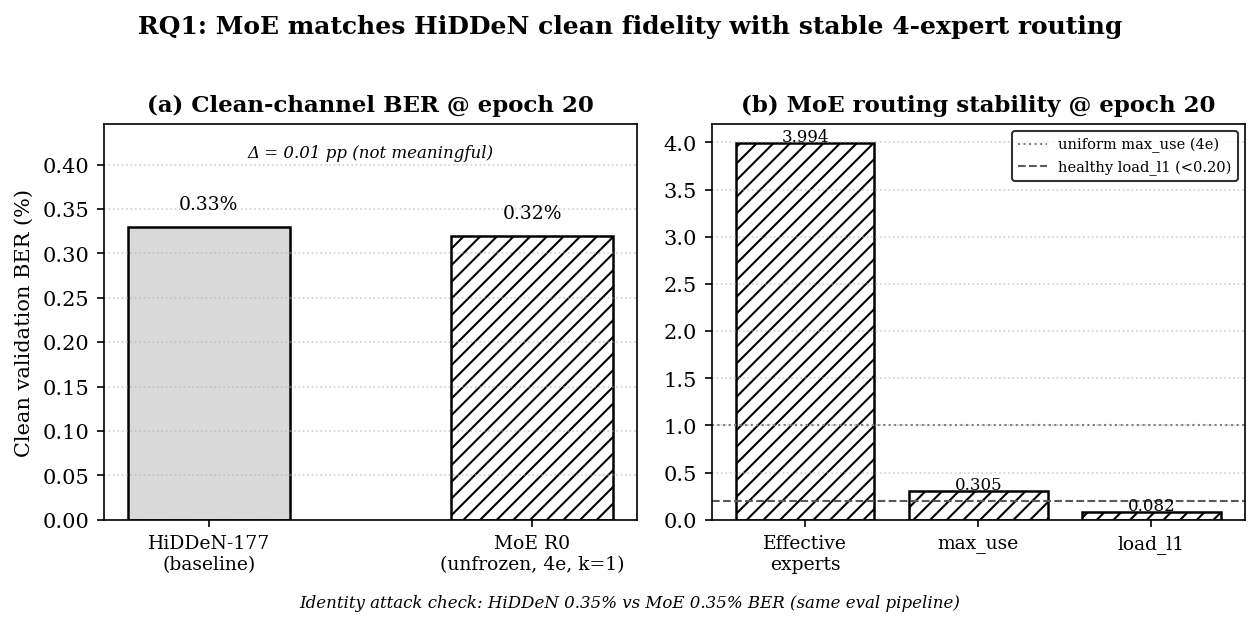
\includegraphics[width=\textwidth]{figures/rq/RQ1_clean_quality.png}
\caption{Experiment 1 results: clean-channel quality comparison. \textit{Left}: bit accuracy distribution across 500 images for both models. \textit{Right}: per-expert validation load at epoch~20; \texttt{expert\_max\_use} $= 0.31$ against a uniform baseline of $0.25$.}
\label{fig:rq1-quality}
\end{figure}

\paragraph{Comments.}
The MoE decoder is statistically indistinguishable from HiDDeN on clean-channel decoding: both reach approximately $99.65\%$ bit accuracy, and encoder MSE is identical. The PSNR gap of roughly 2~dB goes in HiDDeN's favour; I treat this as indicative rather than conclusive given sample size, but it suggests the MoE encoder introduces marginally more distortion. The routing load panel confirms that all four experts are active ($\text{effective experts} \approx 3.99$) with near-uniform load and a small train--validation gap of $0.08$. The practical conclusion is that routing does not degrade clean-channel performance.

%-----

\subsection*{Experiment 2: Robustness Under Image Attacks}
\label{sec:exp2}

\paragraph{Research question.}
Do MoE experts that were routed during clean-channel training generalise better than a single HiDDeN decoder when the watermarked image is subjected to one of eight standard distortions at test time?

\paragraph{Assumptions.}

\begin{table}[H]
\centering
\caption{Fixed and varied parameters for Experiment~2.}
\label{tab:exp2-assumptions}
\begin{tabular}{ll}
\toprule
\textbf{Parameter} & \textbf{Setting} \\
\midrule
HiDDeN checkpoint & epoch-177 \\
MoE checkpoint & R0, epoch-20 \\
Evaluation set & 800 COCO-2017 validation images per attack \\
Attack training & None (both models are clean-trained) \\
Attacks & JPEG Q50, Gaussian noise, crop, cropout, resize, \\
& dropout, quantisation, combined, identity \\
Metric & Bit accuracy (\%) \\
Varied & Attack type; model architecture \\
\bottomrule
\end{tabular}
\end{table}

\paragraph{Course of the experiment.}
For each attack condition, 800 images are encoded by the respective model, the specified distortion is applied to the watermarked image, and the decoder attempts to recover the 30-bit message. The comparison is architecturally controlled: same images, same messages, same attack implementations for both models.

\paragraph{Results.}

\begin{table}[H]
\centering
\caption{Bit accuracy (\%) under each attack condition, 800 images per condition. $\Delta$ is MoE minus HiDDeN. Positive $\Delta$ favours MoE; negative favours HiDDeN. Neither model was trained with these attacks.}
\label{tab:moe-attacks}
\begin{tabular}{lccc}
\toprule
\textbf{Attack} & \textbf{HiDDeN BA (\%)} & \textbf{MoE BA (\%)} & \textbf{$\Delta$ (pp)} \\
\midrule
Gaussian noise & 82.94 & 90.38 & $+7.44$ \\
Crop           & 52.71 & 56.22 & $+3.51$ \\
Cropout        & 85.62 & 89.09 & $+3.47$ \\
Combined       & 50.19 & 50.55 & $+0.37$ \\
Dropout        & 90.59 & 90.63 & $+0.04$ \\
Quantisation   & 99.65 & 99.69 & $+0.04$ \\
None (identity)& 99.65 & 99.65 & $+0.00$ \\
JPEG           & 58.22 & 52.43 & $-5.79$ \\
Resize         & 81.59 & 74.10 & $-7.49$ \\
\bottomrule
\end{tabular}
\end{table}

\begin{figure}[H]
\centering

\includegraphics[width=\textwidth]{figures/rq/RQ2_attack_robustness.png}
\caption{Experiment 2: signed MoE advantage in percentage points per attack. Dark bars (positive) indicate MoE outperforms HiDDeN; light bars (negative) indicate the reverse.}
\label{fig:rq2-robustness}
\end{figure}

\begin{figure}[H]
\centering
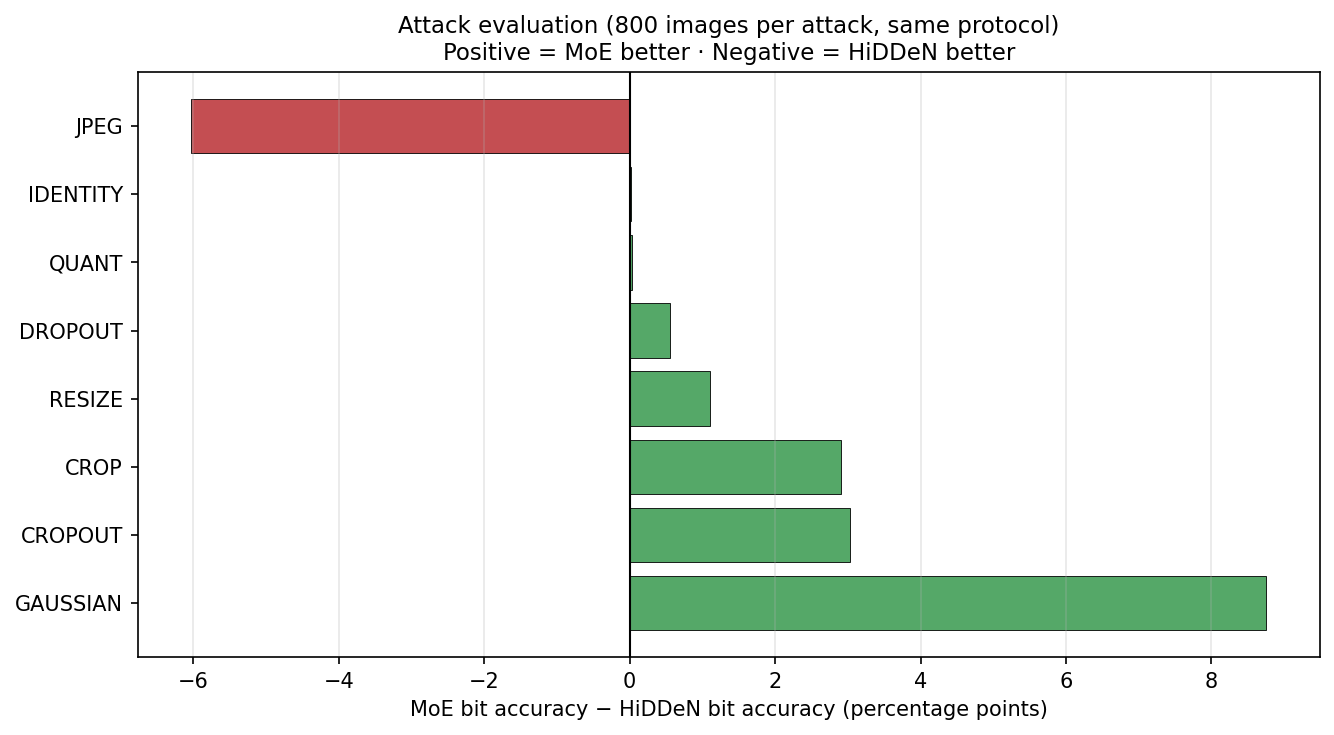
\includegraphics[width=\textwidth]{figures/D_attack_MoE_minus_HiDDeN.png}
\caption{Per-attack bit accuracy comparison with confidence intervals. The advantage on Gaussian noise and crop conditions is consistent across images; the JPEG and resize deficits are also systematic.}
\label{fig:rq2-detail}
\end{figure}

\paragraph{Comments.}
The result is genuinely mixed. Three attacks favour MoE by a meaningful margin: Gaussian noise ($+7.4$~pp), crop ($+3.5$~pp), and cropout ($+3.5$~pp). Four conditions are essentially tied. Two attacks favour HiDDeN: JPEG ($-5.8$~pp) and resize ($-7.5$~pp).

The Gaussian result is the most interpretable: spatially diffuse additive noise has no structural signature, and a routed decoder can dedicate expert capacity to different feature regions, recovering more bits on average. The crop and cropout gains follow a similar logic. The JPEG and resize losses are harder to dismiss---resize's $-7.5$~pp is the largest gap in the table in either direction---and I read them as a training-protocol observation rather than an architectural failure: HiDDeN's original training included JPEG augmentation in some variants, and both distortions involve structured global transformations that a clean-trained router has no reason to align its partition with.

What I want to avoid claiming is that MoE wins on six of nine conditions, because the combined-attack condition, the hardest one, is effectively a coin flip for both models at $\approx 50\%$ BA. Neither architecture has solved multi-distortion robustness from clean training alone.

%------------------------------------------------------------------
\section{Experiment Group 2: Architecture Search (RQ3)}
\label{sec:rq3}
%------------------------------------------------------------------

This group covers the sweep of 26 COCO-100k training runs that led to the reported configuration. All runs use the same training loop, data pipeline, and HiDDeN warm-start; differences are limited to the parameters in each experiment's assumptions table.

The full set of batch-128 runs---the most reliable configurations in the sweep---is presented first, followed by the batch-32 runs that provided specific mechanistic data. Batch-128 runs converge more stably and have lower sensitivity to balance-loss timing, so I treat them as the primary evidence. Table~\ref{tab:ablations-b128} gives the complete batch-128 sweep.

\begin{table}[H]
\centering
\caption{All batch-128 runs on COCO-100k. The reported model (R0) is bold. Lower BER, \texttt{max\_use}, and \texttt{load\_l1} are better. The effective expert count column indicates how many experts are meaningfully active.}
\label{tab:ablations-b128}
\small
\begin{tabular}{lllcccccc}
\toprule
\textbf{Run} & \textbf{BB} & $N$ & $k$ & \textbf{ep} & \textbf{BER (\%)} & \texttt{max\_use} & \texttt{load\_l1} \\
\midrule
\multicolumn{8}{l}{\textit{Backbone comparison (N=4, k=1):}} \\
\textbf{Unfrozen sym\_t14 (R0)} & \textbf{unfrozen} & \textbf{4} & \textbf{1} & \textbf{20} & \textbf{0.32} & \textbf{0.31} & \textbf{0.08} \\
R0 $+$ attack training (ep30) & unfrozen & 4 & 1 & 30 & 0.18 & 0.36 & 0.25 \\
Frozen sym\_bal08 (ep20) & frozen & 4 & 1 & 20 & 2.72 & 0.55 & 0.60 \\
Frozen sym\_bal08 (ep30) & frozen & 4 & 1 & 30 & 7.04 & 0.64 & 0.91 \\
\midrule
\multicolumn{8}{l}{\textit{Routing sparsity k (unfrozen, N=4):}} \\
Unfrozen top-2 ($k=2$) & unfrozen & 4 & 2 & 30 & 2.66 & 0.32 & 0.14 \\
Unfrozen dense ($k=4$) & unfrozen & 4 & 4 & 20 & 2.62 & 0.25 & 0.00 \\
\midrule
\multicolumn{8}{l}{\textit{Expert count N (unfrozen, k=1):}} \\
Unfrozen 8-exp (run A) & unfrozen & 8 & 1 & 20 & 1.70 & 0.30 & 0.53 \\
Unfrozen 8-exp (run B) & unfrozen & 8 & 1 & 20 & 1.36 & 0.51 & 1.11 \\
\midrule
\multicolumn{8}{l}{\textit{Training duration (R0 base):}} \\
R0 continued (ep60) & unfrozen & 4 & 1 & 60 & 4.01 & 0.36 & 0.37 \\
\bottomrule
\end{tabular}
\end{table}

\begin{figure}[H]
\centering
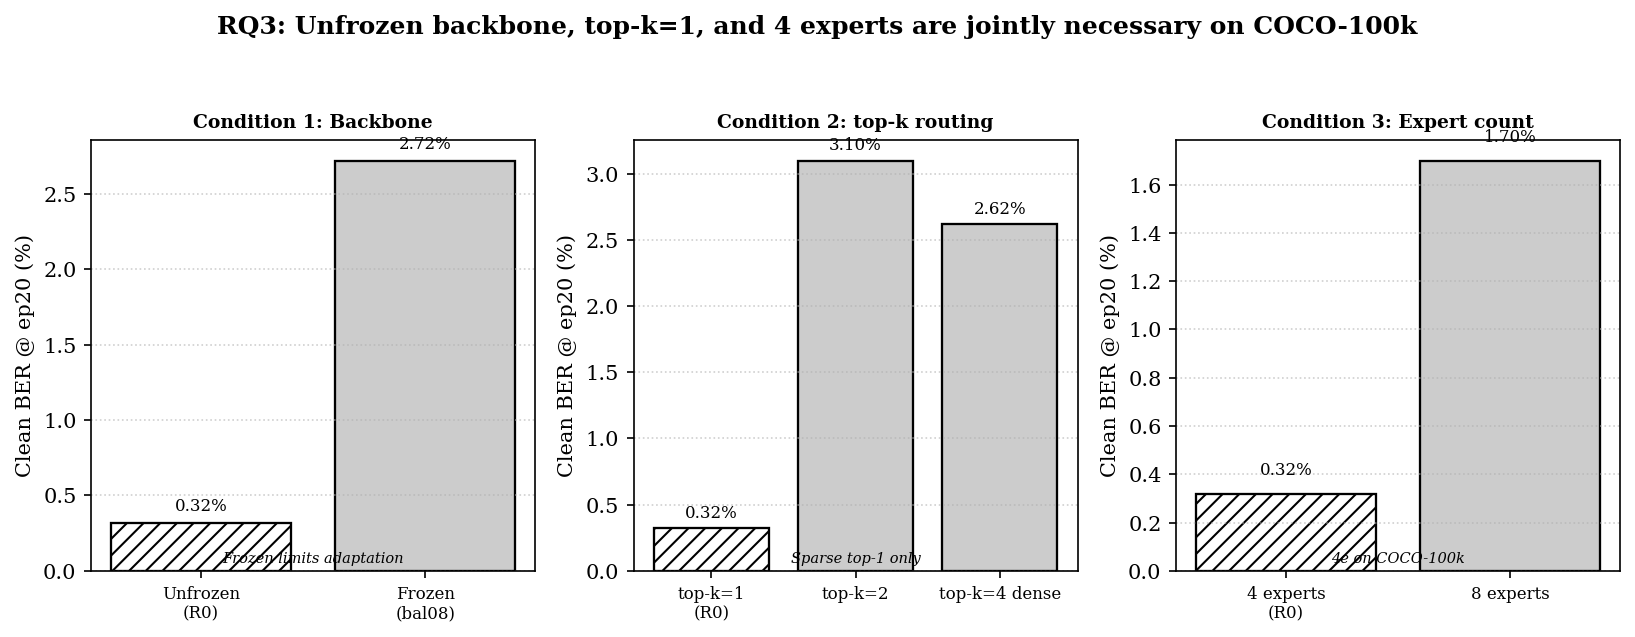
\includegraphics[width=\textwidth]{figures/rq/RQ3_ablation_conditions.png}
\caption{Overview of the batch-128 ablation sweep. Each panel isolates one experimental dimension (backbone, $k$, $N$). The R0 configuration is marked in each. BER and routing collapse score are the primary axes.}
\label{fig:rq3-ablation}
\end{figure}

%-----

\subsection*{Experiment 3: Effect of Backbone Freezing}

\paragraph{Research question.}
Does allowing the HiDDeN encoder and shared convolutional trunk to co-adapt with the routing layer reduce clean-channel BER and routing collapse compared to keeping the backbone frozen?

\paragraph{Assumptions.}

\begin{table}[H]
\centering
\caption{Fixed and varied parameters for Experiment~3.}
\label{tab:exp3-assumptions}
\begin{tabular}{ll}
\toprule
\textbf{Parameter} & \textbf{Setting} \\
\midrule
Primary (batch-128) & $N=4$, $k=1$, batch 128, COCO-100k \\
Secondary (batch-32) & $N=4$, $k=1$, batch 32, COCO-100k \\
Warm-start & HiDDeN epoch-177 \\
Varied & \texttt{freeze\_hidden\_backbone} $\in \{$True, False$\}$ \\
Fixed & $N$, $k$, balance-loss schedule, epochs \\
\bottomrule
\end{tabular}
\end{table}

\paragraph{Course of the experiment.}
Two training runs are compared at batch size 128, differing only in the backbone gradient flag. Routing diagnostics and clean BER are recorded at every epoch; the final values at epoch 20 are the primary comparison point. Batch-32 frozen runs are included as secondary evidence for mechanistic interpretation.

\paragraph{Results.}

\begin{table}[H]
\centering
\caption{Batch-128 frozen vs.\ unfrozen comparison at epoch 20.}
\label{tab:frozen-unfrozen-b128}
\begin{tabular}{llccc}
\toprule
\textbf{Run} & \textbf{Backbone} & \textbf{BER (\%)} & \texttt{max\_use} & \texttt{load\_l1} \\
\midrule
\textbf{R0 (unfrozen, ep20)} & unfrozen & \textbf{0.32} & 0.31 & 0.08 \\
Frozen sym\_bal08 (ep20) & frozen & 2.72 & 0.55 & 0.60 \\
Frozen sym\_bal08 (ep30) & frozen & 7.04 & 0.64 & 0.91 \\
\bottomrule
\end{tabular}
\end{table}

\begin{table}[H]
\centering
\caption{Supporting batch-32 frozen runs providing additional mechanistic data.}
\label{tab:frozen-b32}
\begin{tabular}{llccc}
\toprule
\textbf{Run} & \textbf{Backbone} & \textbf{BER (\%)} & \texttt{max\_use} & \texttt{load\_l1} \\
\midrule
Frozen sym\_t14$\to$0.9 (ep20) & frozen & 0.96 & 0.58 & 1.00 \\
Routing isolation (ep40) & frozen & 0.98 & 1.00 & 1.50 \\
\bottomrule
\end{tabular}
\end{table}

\begin{figure}[H]
\centering
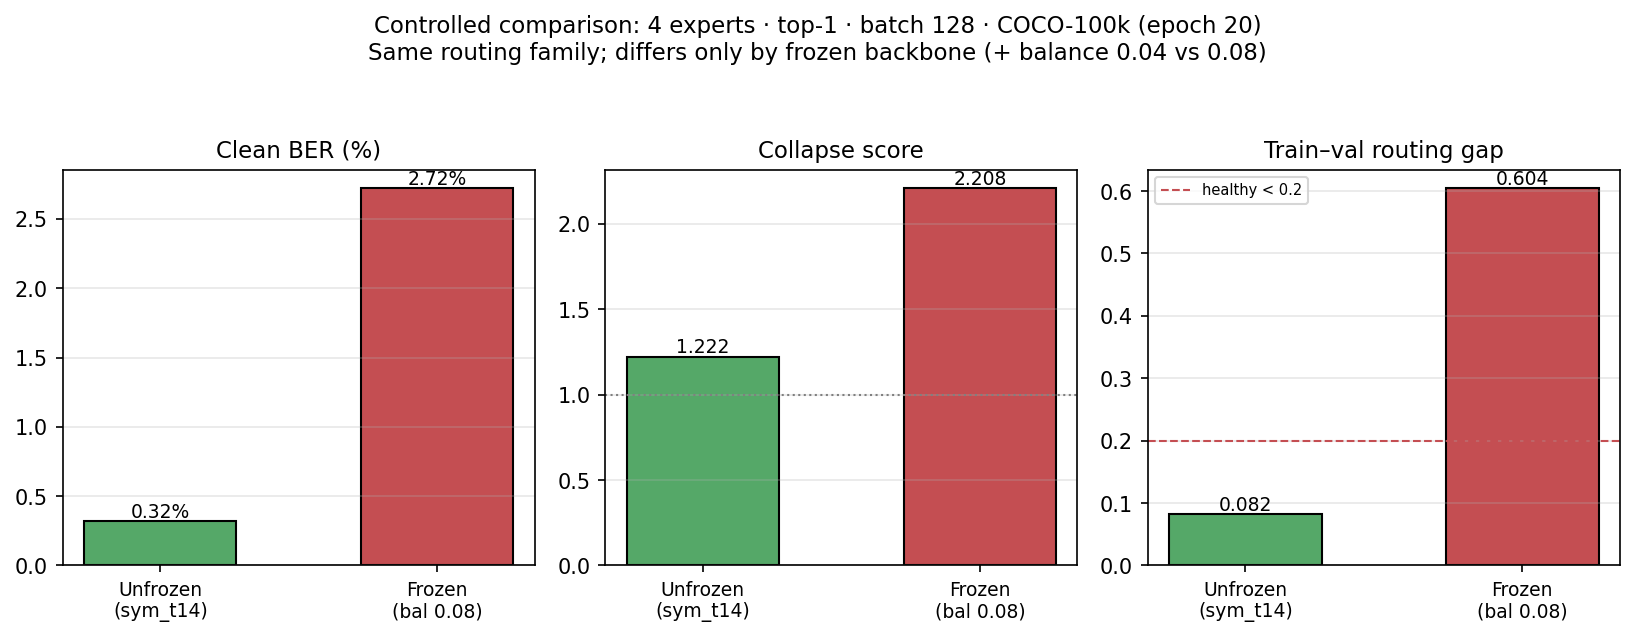
\includegraphics[width=\textwidth]{figures/B_matched_batch128_frozen_vs_unfrozen.png}
\caption{Experiment 3: controlled frozen vs.\ unfrozen comparison (batch 128, $N=4$, $k=1$). \textit{Left}: clean BER. \textit{Centre}: routing collapse score. \textit{Right}: train--validation load gap. Unfreezing reduces all three.}
\label{fig:b128-frozen-vs-unfrozen}
\end{figure}

\begin{figure}[H]
\centering
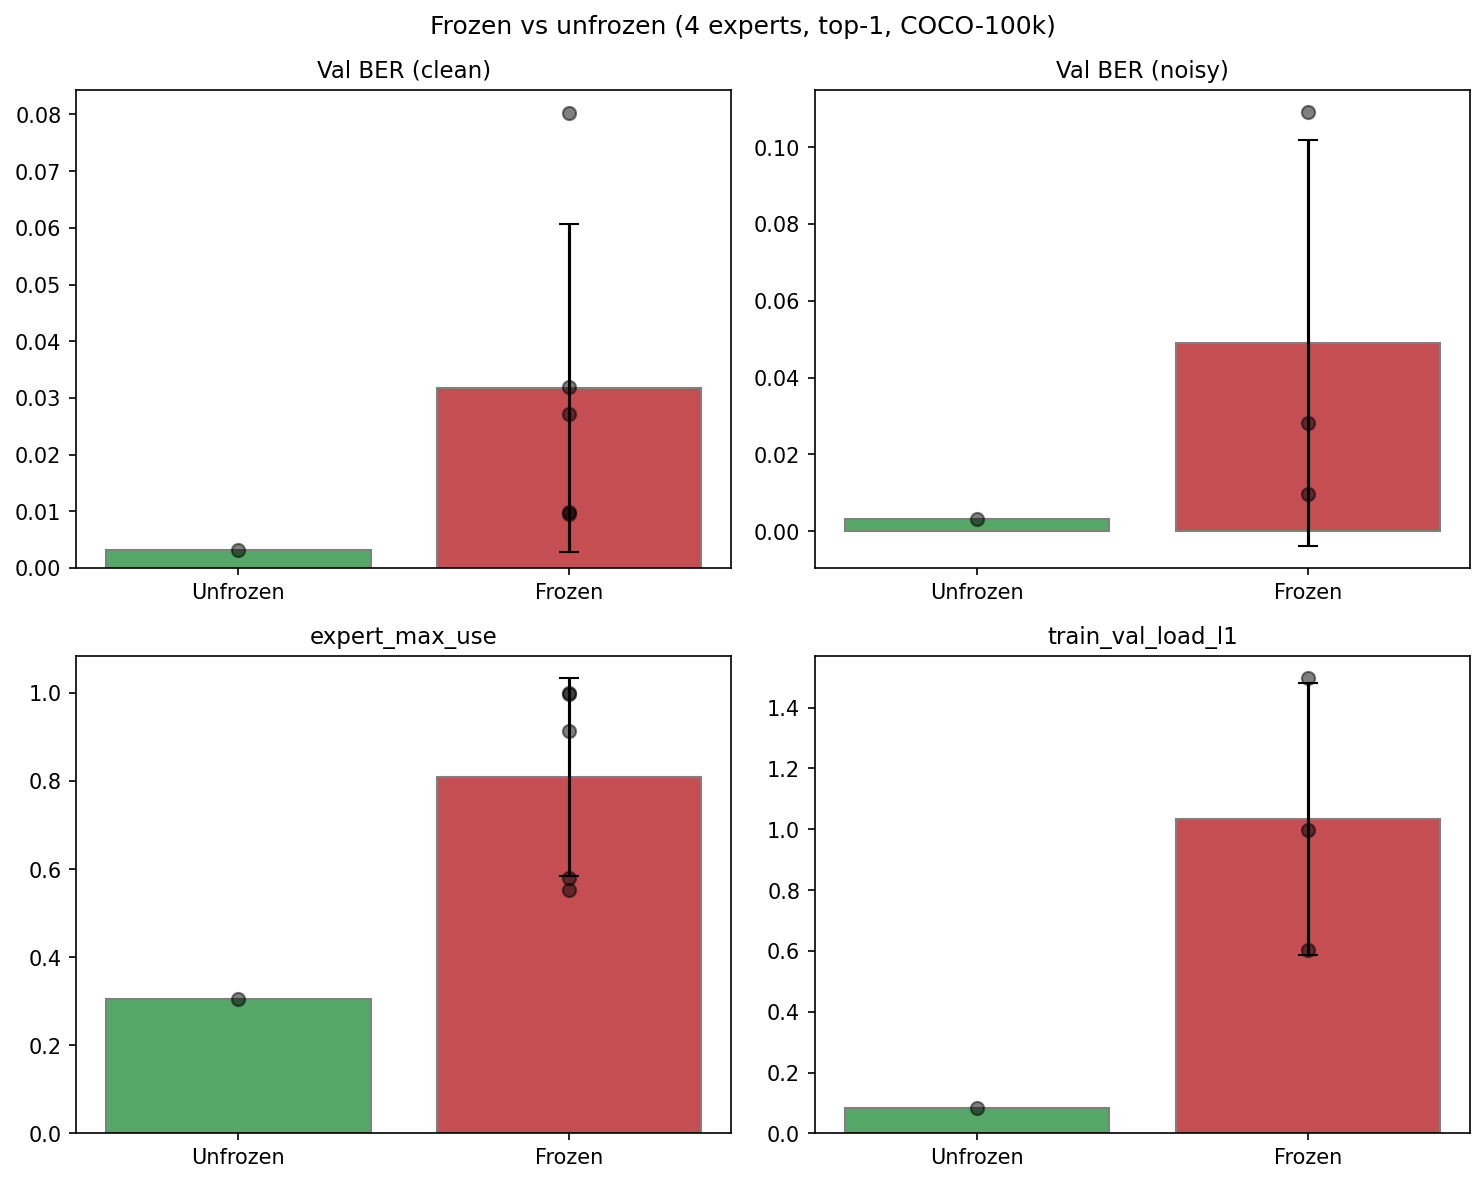
\includegraphics[width=\textwidth]{figures/02_frozen_vs_unfrozen_4exp_k1.png}
\caption{Training curves for frozen and unfrozen backbone runs (batch-32 secondary). BER diverges within the first five epochs: the unfrozen run converges rapidly while the frozen run plateaus at a higher floor.}
\label{fig:frozen-unfrozen-curves}
\end{figure}

\begin{figure}[H]
\centering
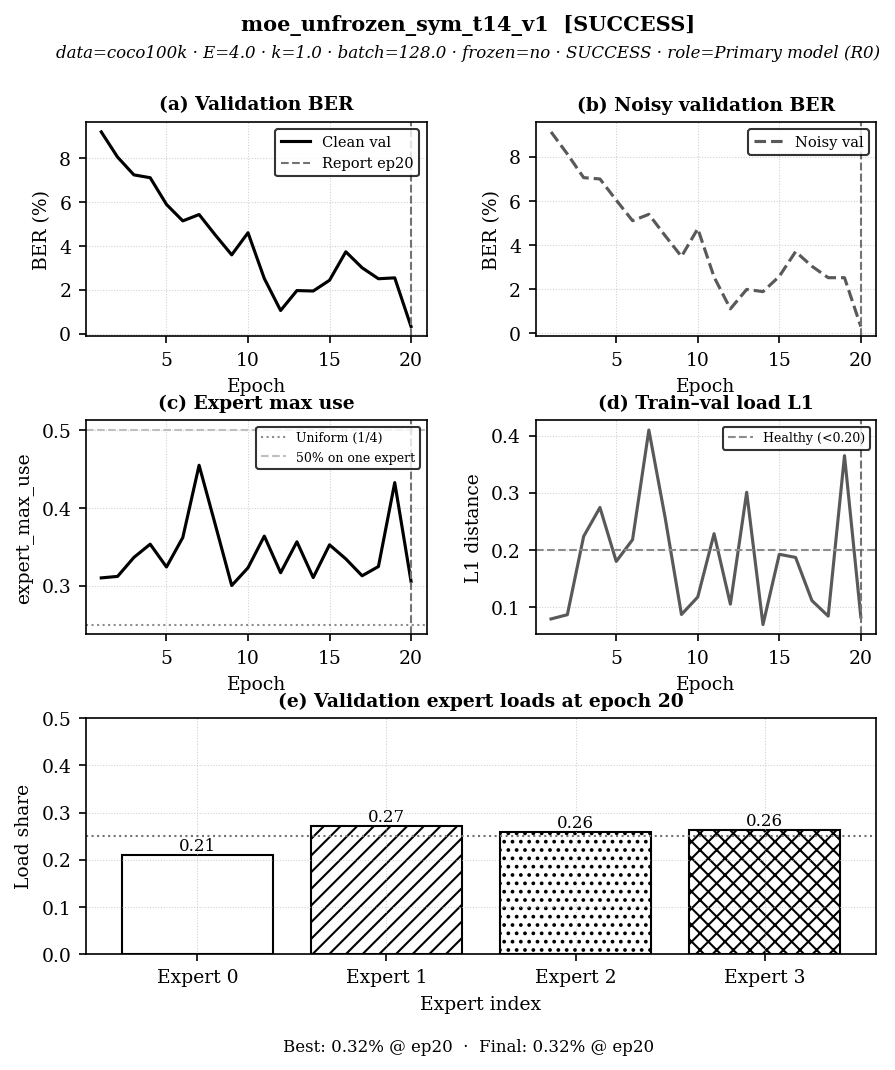
\includegraphics[width=\textwidth]{figures/experiments/01_batch128_sym_t14_unfrozen_bal004warm10_ep20_2026-06-01.png}
\caption{R0 training run (unfrozen, batch 128, epoch 1--20). BER converges to $<1\%$ by epoch 4 and stabilises at $0.32\%$; routing metrics remain healthy throughout.}
\label{fig:r0-curves}
\end{figure}

\begin{figure}[H]
\centering
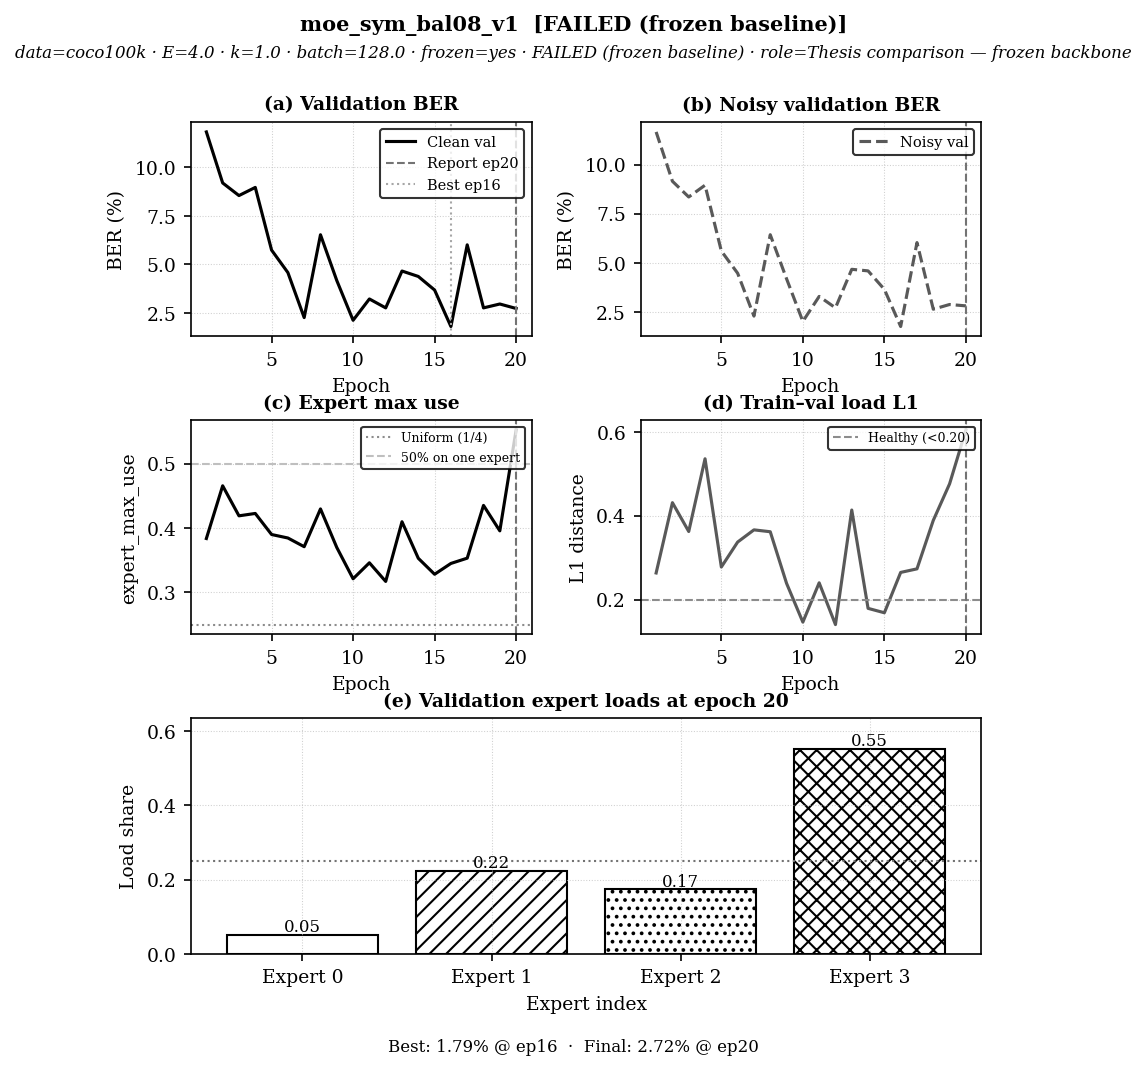
\includegraphics[width=\textwidth]{figures/experiments/28_batch128_sym_bal08_jitter0_bal08warm5_temp14to10_ep20_2026-06-01.png}
\caption{Frozen sym\_bal08 training run (frozen backbone, batch 128, epoch 1--20). BER does not converge below $2\%$ and \texttt{max\_use} climbs, indicating gradual partial collapse.}
\label{fig:frozen-sym-bal08-curves}
\end{figure}

\paragraph{Comments.}
The backbone freezing result is the most decisive finding in the ablation. At batch 128, unfreezing reduces BER from $2.72\%$ to $0.32\%$ and halves the routing collapse score. The frozen run then continues to degrade: by epoch 30 its BER rises to $7.04\%$ and \texttt{max\_use} reaches $0.64$---worse than at epoch 20. That trajectory is not a convergence story, it is a collapse story.

The mechanistic explanation I find convincing is that a frozen backbone gives the router a feature space that was designed for a single decoder, not for a partitioned one. The router must partition representations that were not trained to be separable. When the backbone can adapt, it co-evolves with the routing layer, gradually developing features that genuinely support distinct expert specialisations. The routing isolation run (Table~\ref{tab:frozen-b32}) provides the clearest evidence: 40 epochs of training with a frozen backbone and explicit routing isolation loss produce \texttt{max\_use} $= 1.00$---the router converged to routing every image to the same expert, at which point the MoE is topologically equivalent to a single decoder.

%-----

\subsection*{Experiment 4: Effect of Routing Sparsity ($k$)}

\paragraph{Research question.}
Does allowing each image to be processed by more than one expert ($k > 1$) improve watermark quality, or does it dilute the gradient signal and reduce expert specialisation?

\paragraph{Assumptions.}

\begin{table}[H]
\centering
\caption{Fixed and varied parameters for Experiment~4. All runs: unfrozen, $N=4$, batch 128, COCO-100k.}
\label{tab:exp4-assumptions}
\begin{tabular}{ll}
\toprule
\textbf{Parameter} & \textbf{Setting} \\
\midrule
Backbone & Unfrozen \\
Expert count $N$ & 4 \\
Batch size & 128 \\
Dataset & COCO-100k \\
Varied & $k \in \{1, 2, 4\}$ \\
\bottomrule
\end{tabular}
\end{table}

\paragraph{Course of the experiment.}
Three configurations are trained to convergence (20--30 epochs) and compared on clean BER and routing health. For $k=4$ (dense routing), all four experts contribute to every image in proportion to their router scores.

\paragraph{Results.}

\begin{table}[H]
\centering
\caption{Effect of routing sparsity $k$ on clean-channel BER and routing metrics (unfrozen, $N=4$, batch 128).}
\label{tab:topk-comparison}
\begin{tabular}{cccccc}
\toprule
$k$ & \textbf{ep} & \textbf{BER (\%)} & \texttt{max\_use} & \texttt{load\_l1} & \textbf{Effective exp.} \\
\midrule
1 (R0) & 20 & \textbf{0.32} & 0.31 & 0.08 & 3.99 \\
2      & 30 & 2.66 & 0.32 & 0.14 & --- \\
4      & 20 & 2.62 & 0.25 & 0.00 & 4.00 \\
\bottomrule
\end{tabular}
\end{table}

\begin{figure}[H]
\centering
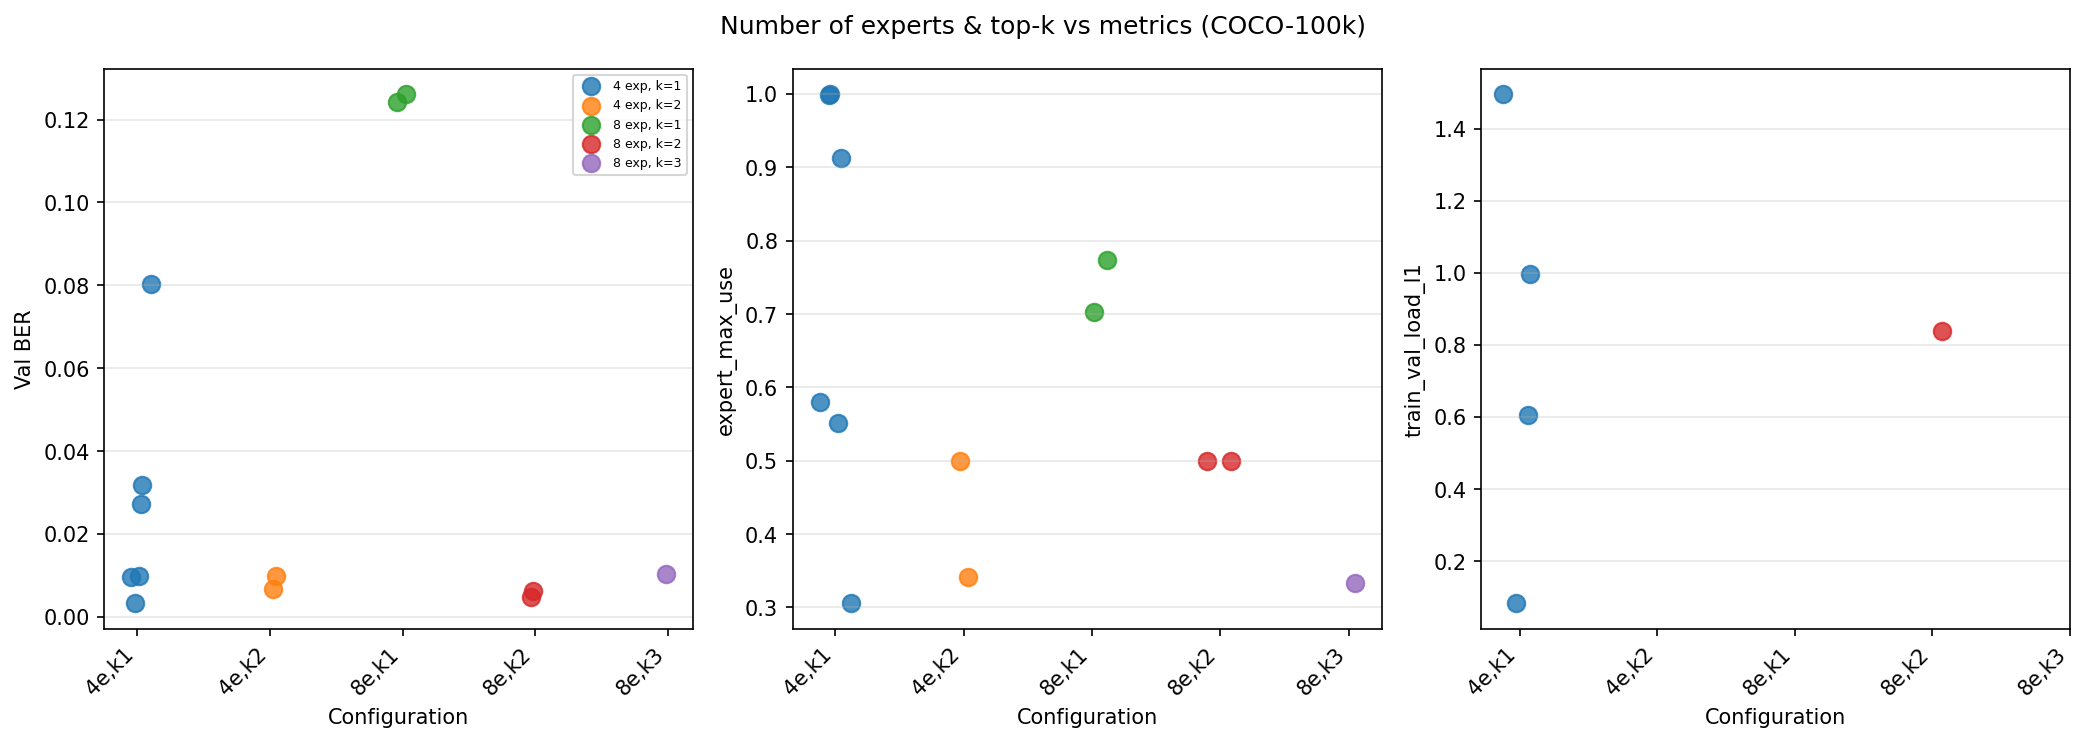
\includegraphics[width=\textwidth]{figures/05_num_experts_topk.png}
\caption{Experiment 4: BER and routing metrics by $k$ (left) and by $N$ (right). Top-1 routing ($k=1$) achieves the lowest BER despite lower expert capacity per image; dense routing ($k=4$) achieves perfect load balance but produces a BER of $2.62\%$.}
\label{fig:topk-nexp}
\end{figure}

\begin{figure}[H]
\centering
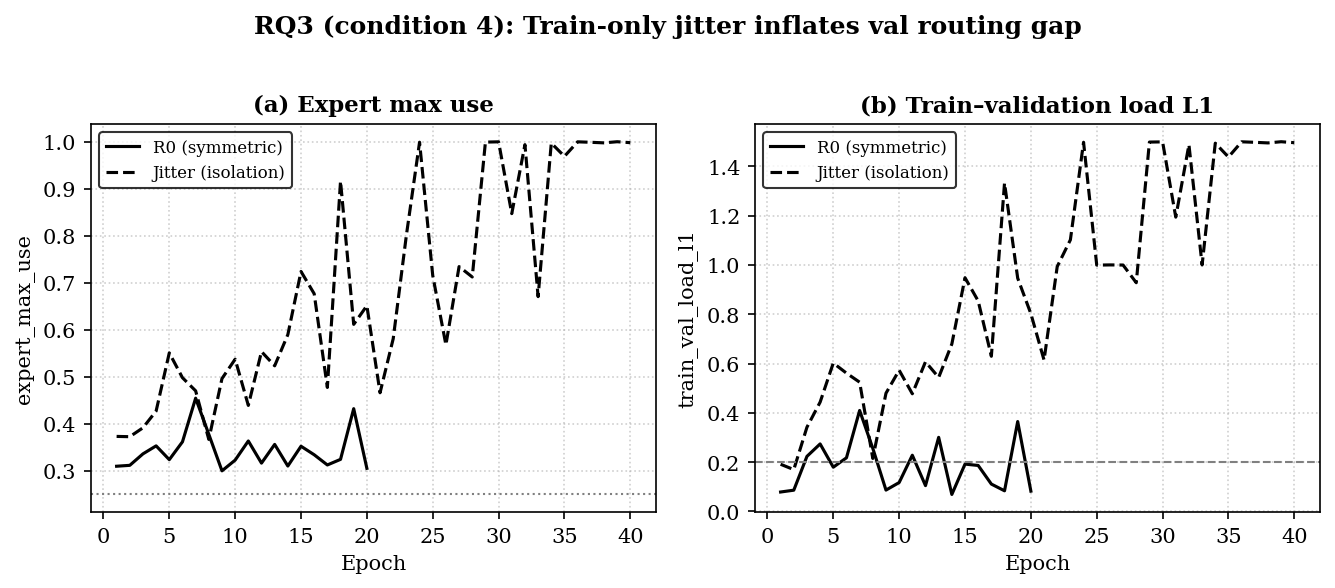
\includegraphics[width=\textwidth]{figures/rq/RQ3_routing_symmetry.png}
\caption{Train and validation expert-load distributions at final epoch for $k \in \{1, 2, 4\}$ (unfrozen, $N=4$). Top-1 routing shows near-perfect train--validation alignment; higher-$k$ runs show increasing generalisation gap.}
\label{fig:routing-symmetry}
\end{figure}

\begin{figure}[H]
\centering
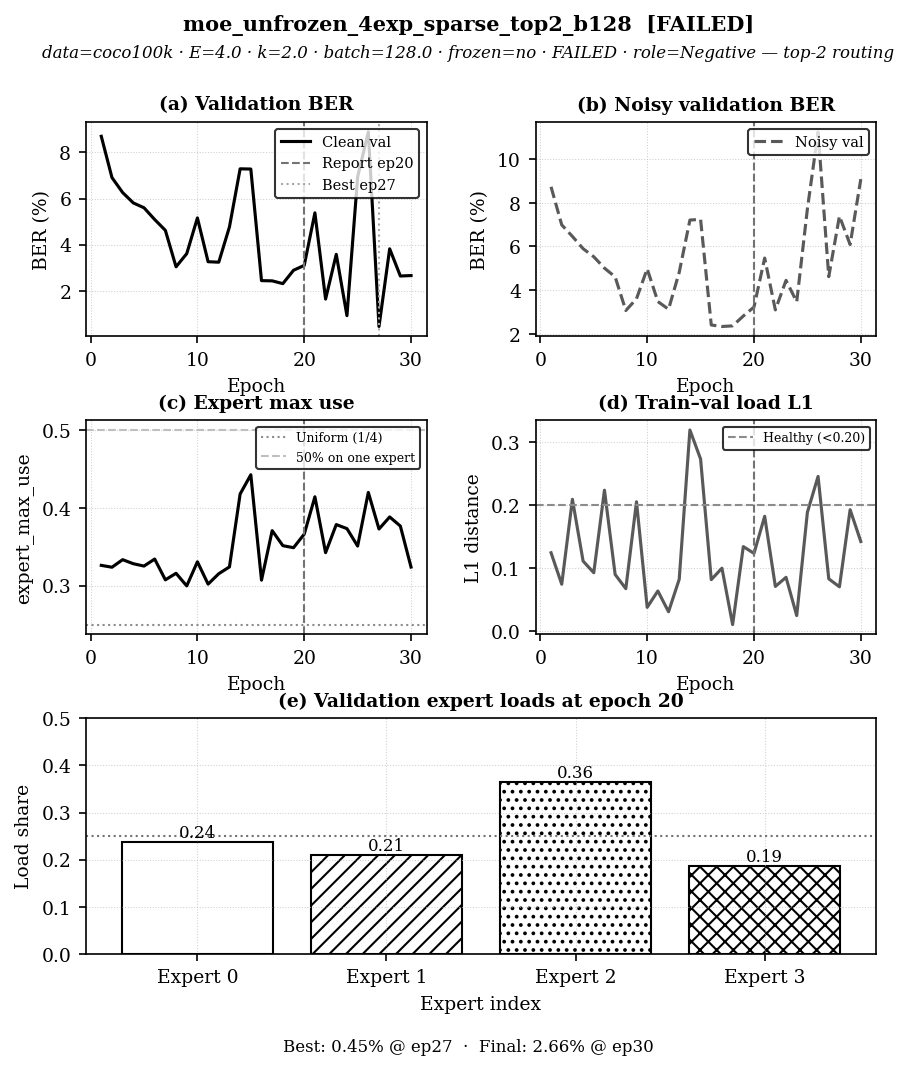
\includegraphics[width=\textwidth]{figures/experiments/24_runs_moe_unfrozen_4exp_sparse_top2_b128_2026_06_03--08-01-13.png}
\caption{Top-2 routing training run ($k=2$, unfrozen, $N=4$, batch 128). BER does not converge below $2\%$ despite 30 epochs; the train--validation routing gap widens steadily.}
\label{fig:top2-curves}
\end{figure}

\paragraph{Comments.}
Top-1 routing outperforms top-2 and top-4 on every metric. This is counterintuitive at first---$k=1$ provides the least expert capacity per image---but becomes clear once you consider the learning dynamics. With top-1 routing, each image is exclusively assigned to one expert, giving that expert clean gradient signal from its assigned subset of the data distribution. With $k=2$, two experts contribute weighted to every image, and each expert receives only a diluted gradient reflecting its contribution fraction. The router learns to hedge rather than specialise.

The $k=4$ (dense) case is the extreme version of this: perfectly uniform \texttt{max\_use} $= 0.25$ and \texttt{load\_l1} $= 0.00$, but BER $= 2.62\%$. The router has learned nothing; every expert contributes equally to every image, and the model is topologically a deep ensemble rather than a mixture. The capacity advantage of four experts is wasted.

%-----

\subsection*{Experiment 5: Effect of Expert Count ($N$)}

\paragraph{Research question.}
Does increasing the number of experts from four to eight improve watermark quality under matched unfrozen training conditions?

\paragraph{Assumptions.}

\begin{table}[H]
\centering
\caption{Fixed and varied parameters for Experiment~5. All runs: unfrozen, $k=1$, batch 128, COCO-100k.}
\label{tab:exp5-assumptions}
\begin{tabular}{ll}
\toprule
\textbf{Parameter} & \textbf{Setting} \\
\midrule
Backbone & Unfrozen \\
Routing $k$ & 1 \\
Batch size & 128 \\
Dataset & COCO-100k \\
Varied & $N \in \{4, 8\}$; two independent 8-exp runs \\
\bottomrule
\end{tabular}
\end{table}

\paragraph{Course of the experiment.}
Three runs are compared: the reported R0 ($N=4$) and two independent 8-expert runs, each trained to epoch 20. The two 8-expert runs allow estimation of run-to-run variance at this setting.

\paragraph{Results.}

\begin{table}[H]
\centering
\caption{Effect of expert count $N$ on BER and routing metrics (unfrozen, $k=1$, batch 128).}
\label{tab:nexp-comparison}
\begin{tabular}{clccc}
\toprule
$N$ & \textbf{Run} & \textbf{BER (\%)} & \texttt{max\_use} & \texttt{load\_l1} \\
\midrule
4 & R0 (ep20) & \textbf{0.32} & 0.31 & 0.08 \\
8 & 8-exp run A (ep20) & 1.70 & 0.30 & 0.53 \\
8 & 8-exp run B (ep20) & 1.36 & 0.51 & 1.11 \\
\bottomrule
\end{tabular}
\end{table}

\begin{figure}[H]
\centering
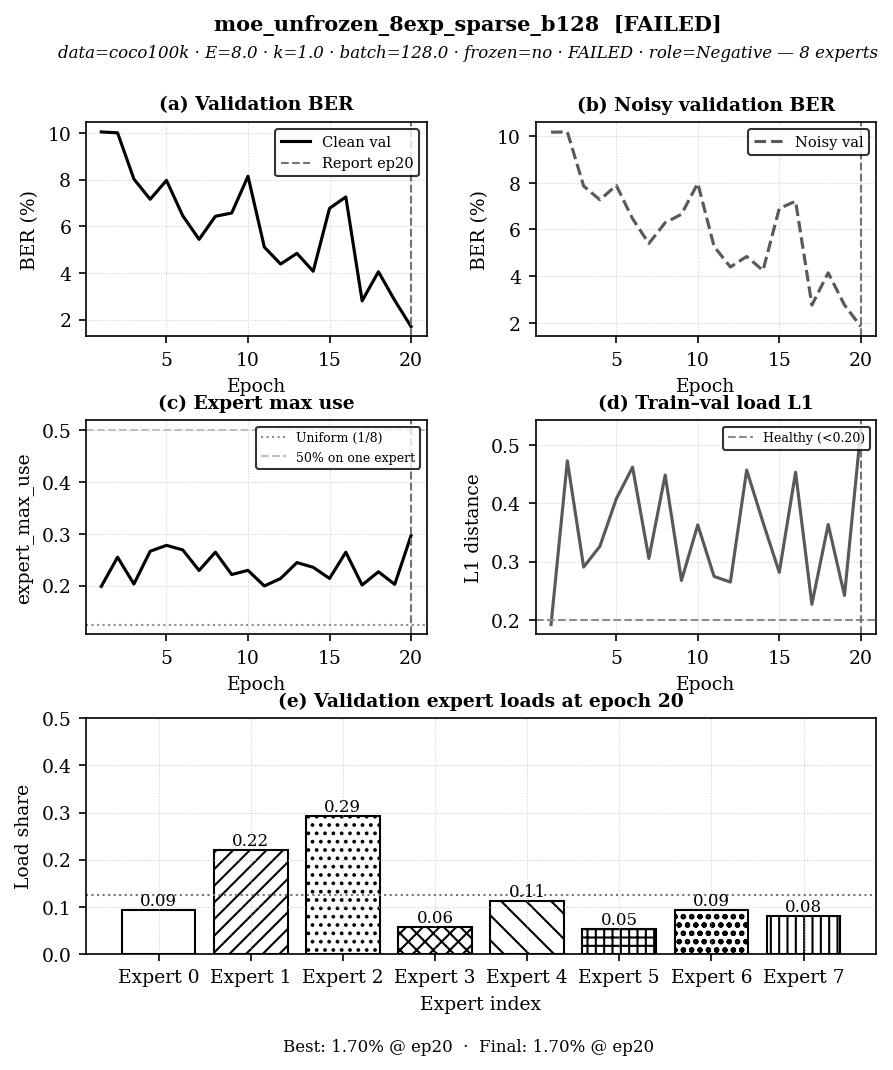
\includegraphics[width=\textwidth]{figures/experiments/25_attack_eval_runs_moe_unfrozen_8exp_sparse_b128_2026_06_02--21-36-20.png}
\caption{8-expert unfrozen run A (batch 128, epoch 1--20). Training BER is competitive but the train--validation routing gap (\texttt{load\_l1} $= 0.53$) is six times larger than R0's.}
\label{fig:8exp-run-a}
\end{figure}

\begin{figure}[H]
\centering
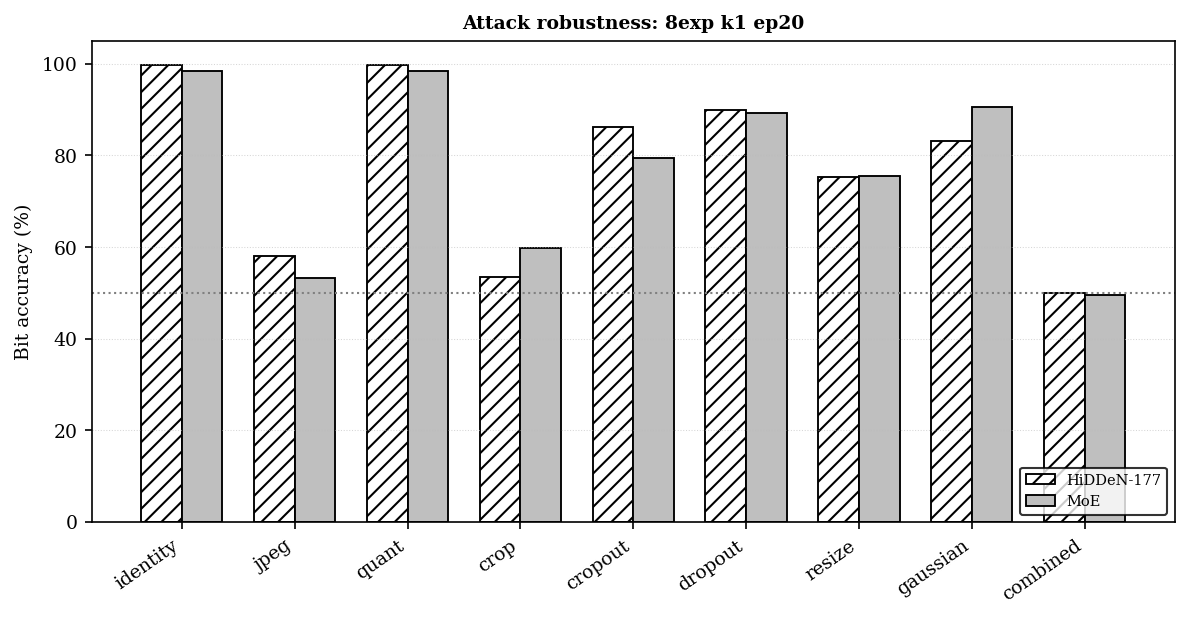
\includegraphics[width=\textwidth]{figures/attacks/atk_8exp_k1_ep20.png}
\caption{Attack evaluation for the 8-expert unfrozen run (run A). Compared to R0, the 8-expert model loses ground on JPEG and resize by wider margins while retaining the Gaussian-noise advantage.}
\label{fig:8exp-attacks}
\end{figure}

\paragraph{Comments.}
Eight experts is strictly worse than four at this dataset scale. Run A reaches BER $1.70\%$ with \texttt{load\_l1} $= 0.53$; run B reaches $1.36\%$ but with \texttt{load\_l1} $= 1.11$---a routing gap eleven times larger than R0. The healthy \texttt{max\_use} values in both runs (0.30 and 0.51 respectively) initially suggest the experts are not collapsed, but the large routing gap tells the real story: the router learned a partition of the training distribution that did not generalise. Run-to-run variance is also substantial: BER differs by $0.34$~pp and \texttt{load\_l1} by $0.58$ between the two identical runs, which suggests the 8-expert configuration is at or near the edge of what this dataset can support.

My interpretation is that COCO-100k does not contain enough diversity, or is not diverse in the right way, to justify eight specialised experts. With four experts, each one is assigned roughly 29{,}500 training images on average; with eight, that drops to roughly 14{,}750, and the expert representations become under-specified. The correct answer may be to use eight experts on a larger or more semantically diverse corpus.

%-----

\subsection*{Experiment 6: Effect of Training Duration}

\paragraph{Research question.}
Does extending training beyond 20 epochs improve the R0 configuration, or does longer training cause the routing gap to widen?

\paragraph{Assumptions.}

\begin{table}[H]
\centering
\caption{Fixed and varied parameters for Experiment~6.}
\label{tab:exp6-assumptions}
\begin{tabular}{ll}
\toprule
\textbf{Parameter} & \textbf{Setting} \\
\midrule
Checkpoint base & R0 epoch-20 \\
Training resumed & 40 additional epochs (epochs 21--60) \\
Architecture & Same as R0 ($N=4$, $k=1$, unfrozen, batch 128) \\
Varied & Number of training epochs \\
\bottomrule
\end{tabular}
\end{table}

\paragraph{Course of the experiment.}
The R0 epoch-20 checkpoint is resumed with the same learning rate, balance-loss weight, and temperature schedule. Validation BER and routing metrics are logged at every epoch. Two additional early-stopped checkpoints (ep22 and ep26) were manually extracted and tested for comparison.

\paragraph{Results.}

\begin{table}[H]
\centering
\caption{Validation BER and routing gap at selected checkpoints from the R0 continuation run.}
\label{tab:duration-comparison}
\begin{tabular}{ccccc}
\toprule
\textbf{Epoch} & \textbf{BER (\%)} & \texttt{max\_use} & \texttt{load\_l1} & \textbf{Note} \\
\midrule
20 (R0) & \textbf{0.32} & 0.31 & 0.08 & Reported model \\
22 & 0.14 & 0.33 & 0.12 & Briefly better BER \\
26 & 0.09 & 0.34 & 0.16 & Briefly better BER \\
30 & 0.38 & 0.35 & 0.22 & BER regressing \\
60 & 4.01 & 0.36 & 0.37 & Substantial degradation \\
\bottomrule
\end{tabular}
\end{table}

\begin{figure}[H]
\centering
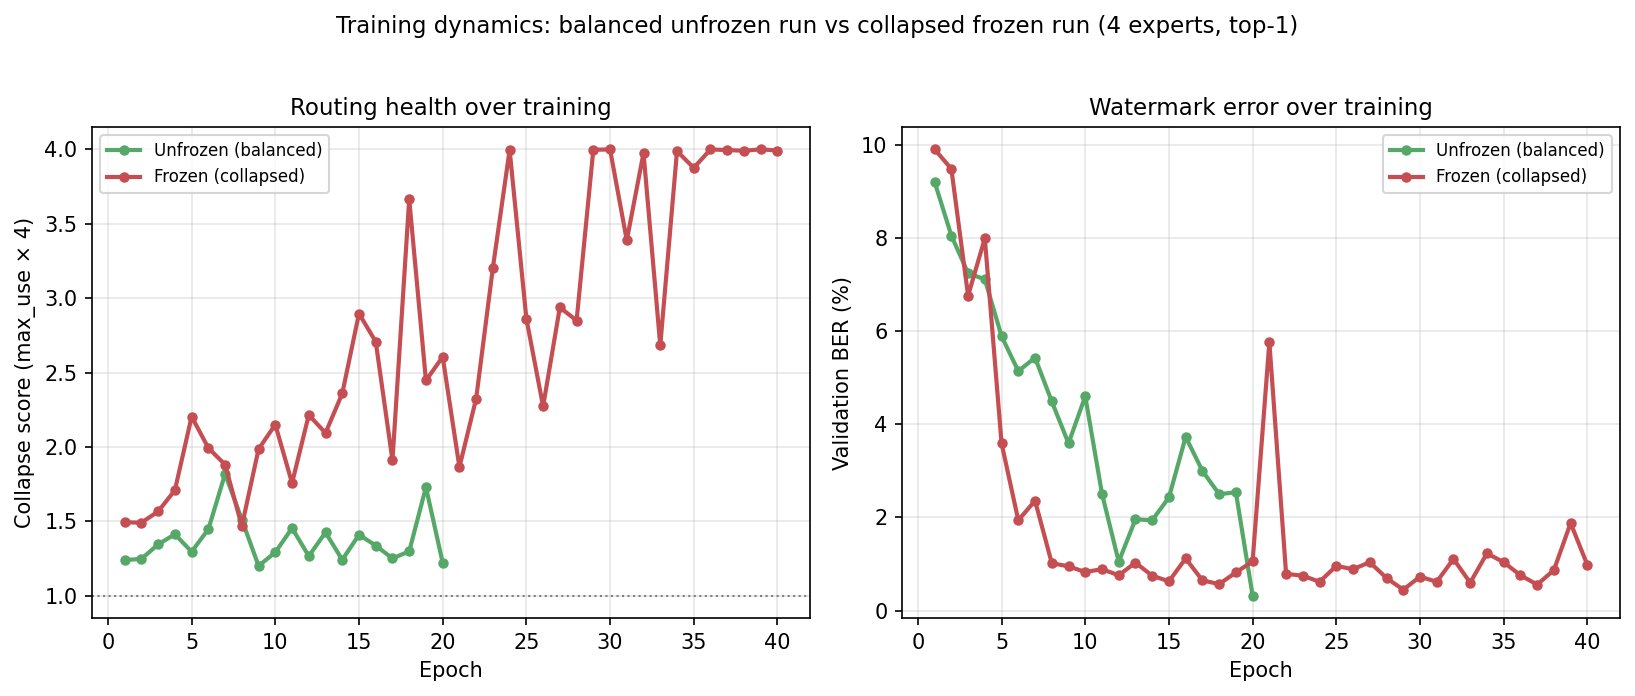
\includegraphics[width=\textwidth]{figures/C_training_collapse_and_BER_over_epochs.png}
\caption{Experiment 6: BER and routing collapse over training epochs for R0 (continued beyond epoch 20). BER briefly improves at epochs 22--26 before degrading; the train--validation routing gap widens monotonically.}
\label{fig:duration-curves}
\end{figure}

\begin{figure}[H]
\centering
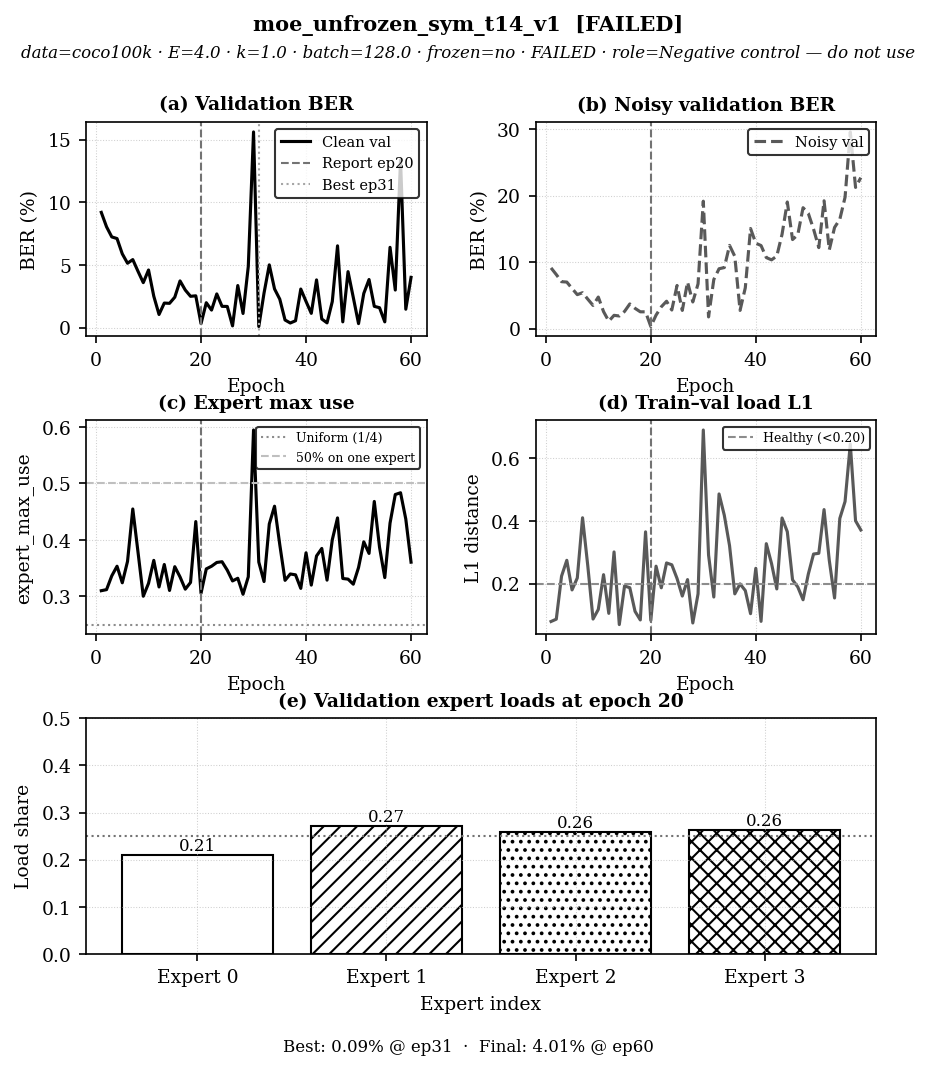
\includegraphics[width=\textwidth]{figures/experiments/27_exp4continue_extracted_moe_unfrozen_sym_t14_v1_continue.png}
\caption{Extended R0 continuation run (epochs 1--60). The clean-channel BER valley at epoch 20 is visible; the degradation from epoch 30 onwards is systematic, not noisy.}
\label{fig:r0-continuation}
\end{figure}

\paragraph{Comments.}
Early stopping at epoch 20 is the right choice, but it is not a lucky stopping point. The continuation data shows that BER briefly dips below R0's epoch-20 value at epochs 22 and 26---the model does improve marginally if you use a late-epoch oracle. What makes epoch 20 the practical choice is the routing gap: at epoch 20, \texttt{load\_l1} $= 0.08$; by epoch 26 it has already risen to $0.16$; by epoch 60 it is $0.37$. No BER gain is worth a fourfold increase in routing fragility. The routing gap is the early warning sign; the BER degradation follows later.

%------------------------------------------------------------------
\section{Experiment Group 3: Inference Cost (RQ4)}
\label{sec:rq4}
%------------------------------------------------------------------

\subsection*{Experiment 7: Latency and Peak Memory Benchmark}

\paragraph{Research question.}
What is the per-image inference latency and peak GPU memory of the MoE decoder relative to HiDDeN, and does the overhead converge at realistic batch sizes?

\paragraph{Assumptions.}

\begin{table}[H]
\centering
\caption{Fixed and varied parameters for Experiment~7.}
\label{tab:exp7-assumptions}
\begin{tabular}{ll}
\toprule
\textbf{Parameter} & \textbf{Setting} \\
\midrule
HiDDeN checkpoint & epoch-177 \\
MoE checkpoint & R0 epoch-20 with sparse conditional dispatch \\
GPU & NVIDIA (same device for both; CUDA 12.8) \\
Warmup passes & 10 (discarded) \\
Timed passes & 50 (averaged) \\
Dispatch mode & Sparse conditional (only the routed expert executes) \\
Varied & Batch size $\in \{1, 8, 32\}$; model \\
\bottomrule
\end{tabular}
\end{table}

\paragraph{Course of the experiment.}
Each model is loaded with \texttt{torch.no\_grad()} active. After 10 warmup passes to prime CUDA caches, 50 encode--decode passes are timed with \texttt{torch.cuda.Event} synchronisation. Peak memory is measured with \texttt{torch.cuda.max\_memory\_allocated()}. The MoE decoder uses the sparse dispatch implementation described in Chapter~3: at batch size 1, top-1 routing activates exactly one expert and skips the other three.

\paragraph{Results.}

\begin{table}[H]
\centering
\caption{Inference latency (ms per image) and peak GPU memory. \textit{enc} = encode only; \textit{dec} = decode only; \textit{full} = encode + decode. Dec.\ ratio is MoE/HiDDeN on the decode step only.}
\label{tab:moe-cost}
\small
\begin{tabular}{lcrrrrc}
\toprule
\textbf{Model} & \textbf{Batch} & \textbf{enc (ms/img)} & \textbf{dec (ms/img)} & \textbf{full (ms/img)} & \textbf{mem (MB)} & \textbf{dec ratio} \\
\midrule
HiDDeN & 1  & 0.81 & 1.04 & 1.80 & 72.7  & 1.00$\times$ \\
MoE    & 1  & 0.82 & 10.01 & 15.78 & 76.3 & 9.59$\times$ \\
\midrule
HiDDeN & 8  & 1.04 & 1.35 & 2.32 & 246.8  & 1.00$\times$ \\
MoE    & 8  & 1.03 & 2.62 & 3.60 & 256.2  & 1.94$\times$ \\
\midrule
HiDDeN & 32 & 0.99 & 1.32 & 2.29 & 843.8  & 1.00$\times$ \\
MoE    & 32 & 0.99 & 2.17 & 3.12 & 843.8  & \textbf{1.64$\times$} \\
\bottomrule
\end{tabular}
\end{table}

\begin{figure}[H]
\centering
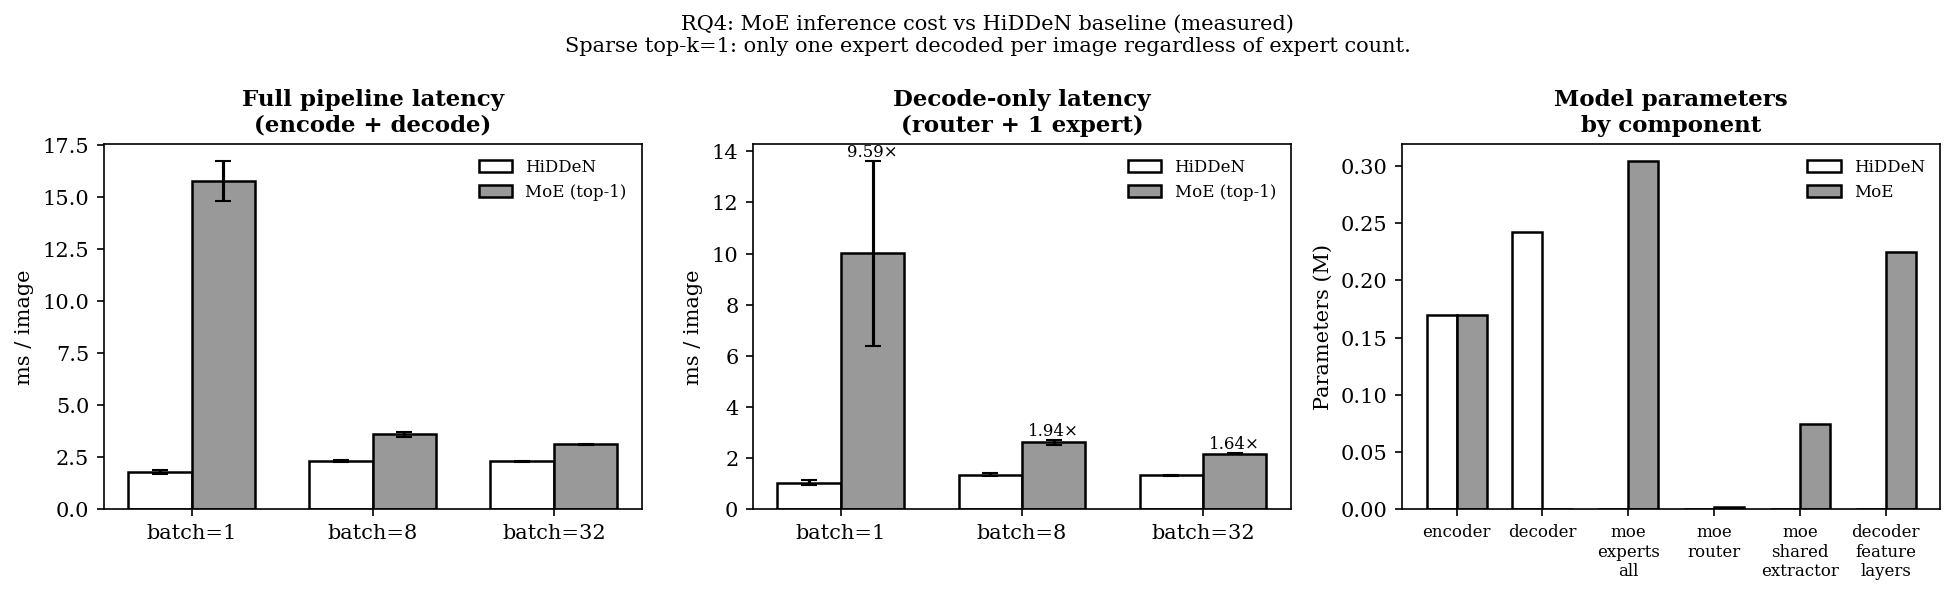
\includegraphics[width=\textwidth]{figures/rq/RQ4_inference_cost.png}
\caption{Experiment 7: full-pipeline latency per image at batch sizes 1, 8, and 32 (left); decode overhead ratio (centre); parameter count breakdown (right). The batch=1 spike is a Python dispatch artefact, not a GPU bottleneck.}
\label{fig:rq4-cost}
\end{figure}

\paragraph{Comments.}
The encoder timings are identical: both models share the same encoder, so the $0.99$ ms/image at batch 32 is exactly the same for both. All cost difference lives in the decoder.

At batch 32, the decode overhead is $1.64\times$ and the full-pipeline overhead is $1.36\times$, with identical peak memory. The batch=1 decode ratio of $9.59\times$ is a Python-level artefact: iterating over four experts, computing boolean dispatch masks, and launching conditional CUDA kernels each carry fixed overhead that does not amortise at a single image. The overhead converges quickly: $1.94\times$ at batch 8, $1.64\times$ at batch 32. The memory penalty is negligible ($76.3$ vs $72.7$~MB at batch 1).

Parameter counts: HiDDeN has 411{,}903 parameters; MoE R0 has 774{,}175---a $1.88\times$ increase, all on the decoder side. The four experts share the same shared trunk and add four independent prediction heads; neither the encoder nor the discriminator gains any parameters.

%------------------------------------------------------------------
\section{Experiment Group 4: Routing Collapse as a Failure Predictor (RQ5)}
\label{sec:rq5}
%------------------------------------------------------------------

\subsection*{Experiment 8: Collapse--BER Correlation Across the Full Sweep}

\paragraph{Research question.}
Does the routing collapse score (\texttt{expert\_max\_use}) measured at the end of training predict final clean-channel BER across all COCO-100k runs, and can it serve as a mid-training early-stopping criterion?

\paragraph{Assumptions.}

\begin{table}[H]
\centering
\caption{Fixed and varied parameters for Experiment~8.}
\label{tab:exp8-assumptions}
\begin{tabular}{ll}
\toprule
\textbf{Parameter} & \textbf{Setting} \\
\midrule
Run set & All COCO-100k runs with full validation logs ($n = 13$) \\
Collapse metric & \texttt{expert\_max\_use} (final epoch) \\
Outcome metric & Validation BER (\%) (final epoch) \\
Statistical test & Pearson $r$ and two-tailed $p$-value \\
Varied & Architecture, backbone, $k$, $N$ (full sweep) \\
\bottomrule
\end{tabular}
\end{table}

\paragraph{Course of the experiment.}
Final-epoch routing diagnostics and validation BER are extracted from the logging CSV of each completed COCO-100k run. Pearson correlation is computed between \texttt{expert\_max\_use} and BER. Training-dynamics curves are plotted for representative healthy and collapsed runs to assess whether collapse is an early or late phenomenon. Failure modes are classified manually based on the collapse score, routing gap, and BER trajectory.

\paragraph{Results.}

\begin{table}[H]
\centering
\caption{Routing diagnostic summary for three representative configurations. For $N=4$ experts, perfect uniformity gives \texttt{max\_use} $= 0.25$.}
\label{tab:moe-routing}
\begin{tabular}{lcccc}
\toprule
\textbf{Configuration} & \texttt{max\_use} & \texttt{load\_l1} & \textbf{BER (\%)} & \textbf{Status} \\
\midrule
Unfrozen sym\_t14 (R0) & 0.31 & 0.08 & 0.32 & Healthy \\
Frozen sym\_bal08 (ep20) & 0.55 & 0.60 & 2.72 & Partial collapse \\
Routing isolation (ep40) & 1.00 & 1.50 & 0.98 & Full collapse \\
\bottomrule
\end{tabular}
\end{table}

\begin{figure}[H]
\centering

\includegraphics[width=\textwidth]{figures/rq/collapse_vs_ber_all_runs.png}
\caption{Experiment 8: routing collapse versus clean-channel BER across all 28 training runs. \textit{(a)} COCO-100k runs only ($n=20$): Pearson $r=0.63$, $p=0.003$ — a clear positive trend. \textit{(b)} All 28 runs: correlation weakens to $r=0.29$ because COCO-20k exploratory runs (orange squares) show low collapse scores but very high BER, a different failure mode driven by insufficient training data. \textit{(c)} Strip plot by failure-mode category; horizontal lines are medians. Healthy unfrozen runs cluster below 2\%, partial collapse sits around 1--3\%, full collapse around 1\%, and small-dataset runs span 0.5--21\%.}
\label{fig:rq5-scatter}
\end{figure}

\begin{figure}[H]
\centering
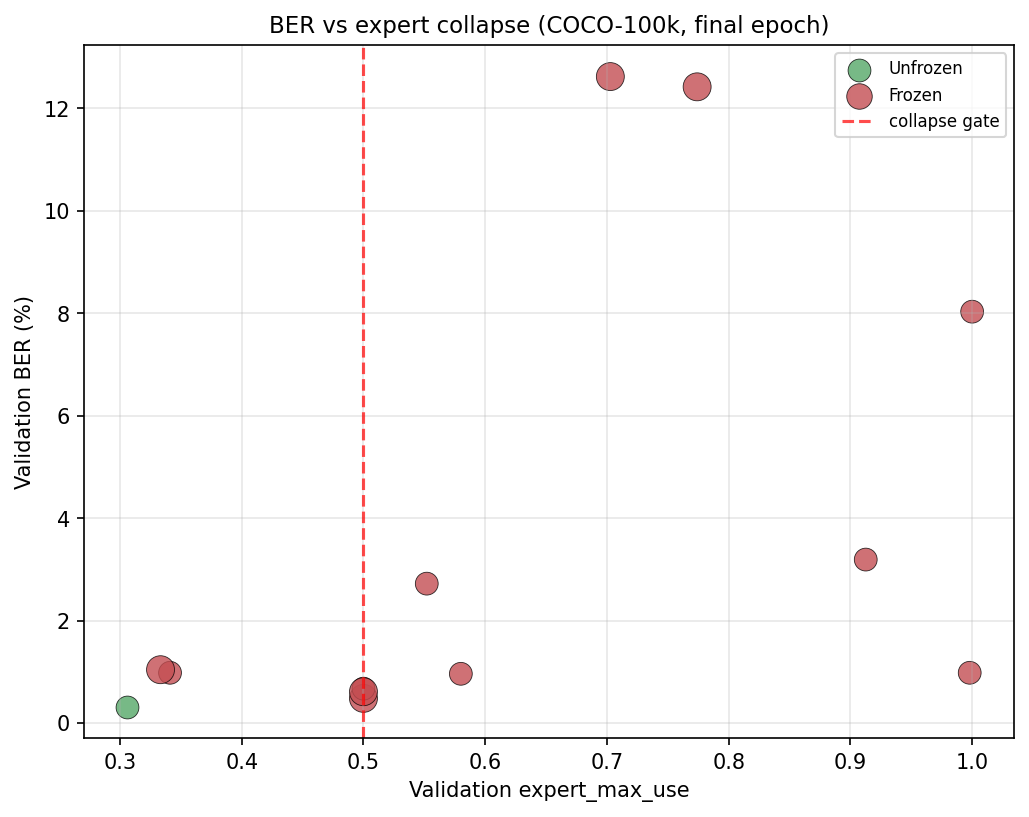
\includegraphics[width=\textwidth]{figures/07_ber_vs_expert_max_use.png}
\caption{BER vs.\ \texttt{expert\_max\_use} for all COCO-100k runs, with backbone type annotated. The relationship is systematic but not deterministic: a healthy routing score is necessary but not sufficient for low BER.}
\label{fig:ber-vs-maxuse}
\end{figure}

\begin{figure}[H]
\centering
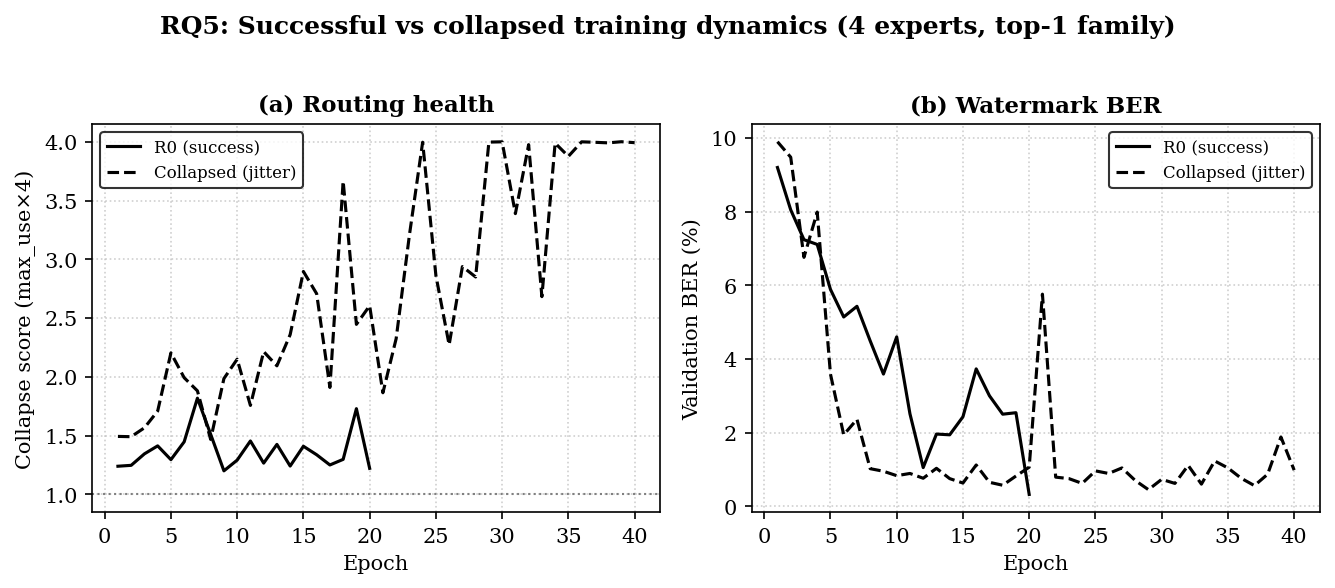
\includegraphics[width=\textwidth]{figures/rq/RQ5_training_dynamics.png}
\caption{Training dynamics across epochs for R0 (healthy) and a representative collapsed frozen run. \textit{Left}: collapse score over epochs. \textit{Right}: validation BER. Collapse establishes itself within the first five epochs; BER divergence follows shortly after.}
\label{fig:rq5-dynamics}
\end{figure}

\begin{figure}[H]
\centering
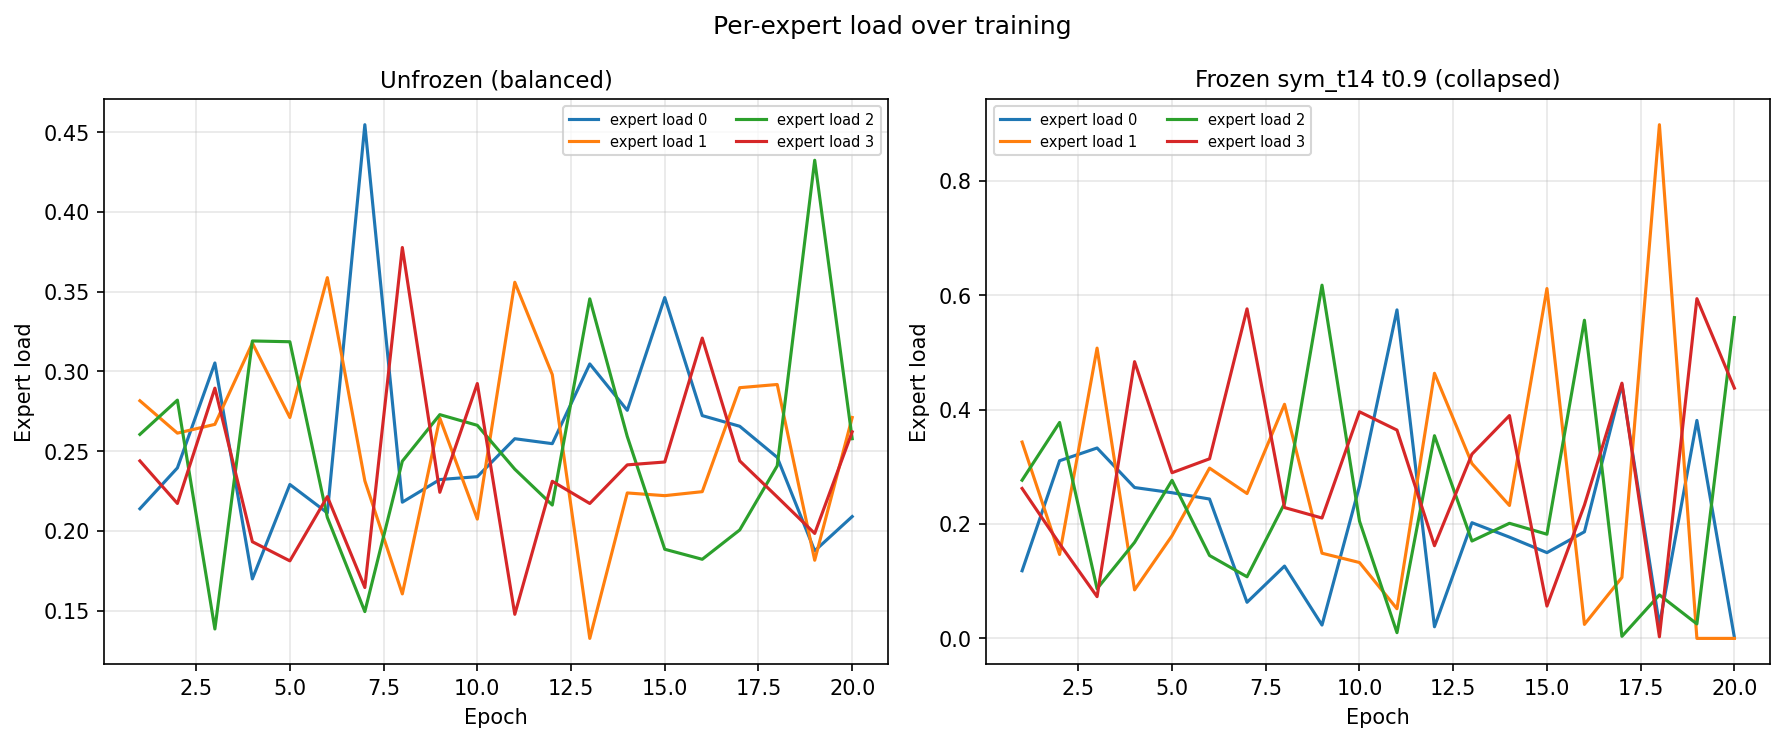
\includegraphics[width=\textwidth]{figures/11_expert_load_over_epochs.png}
\caption{Per-expert load fractions over training for the R0 run (top) and a partially collapsed frozen run (bottom). R0's four experts stabilise near $0.25$ load each by epoch 5; the frozen run's two dominant experts absorb increasing fractions of traffic from epoch 3 onwards.}
\label{fig:expert-load-epochs}
\end{figure}

\begin{figure}[H]
\centering
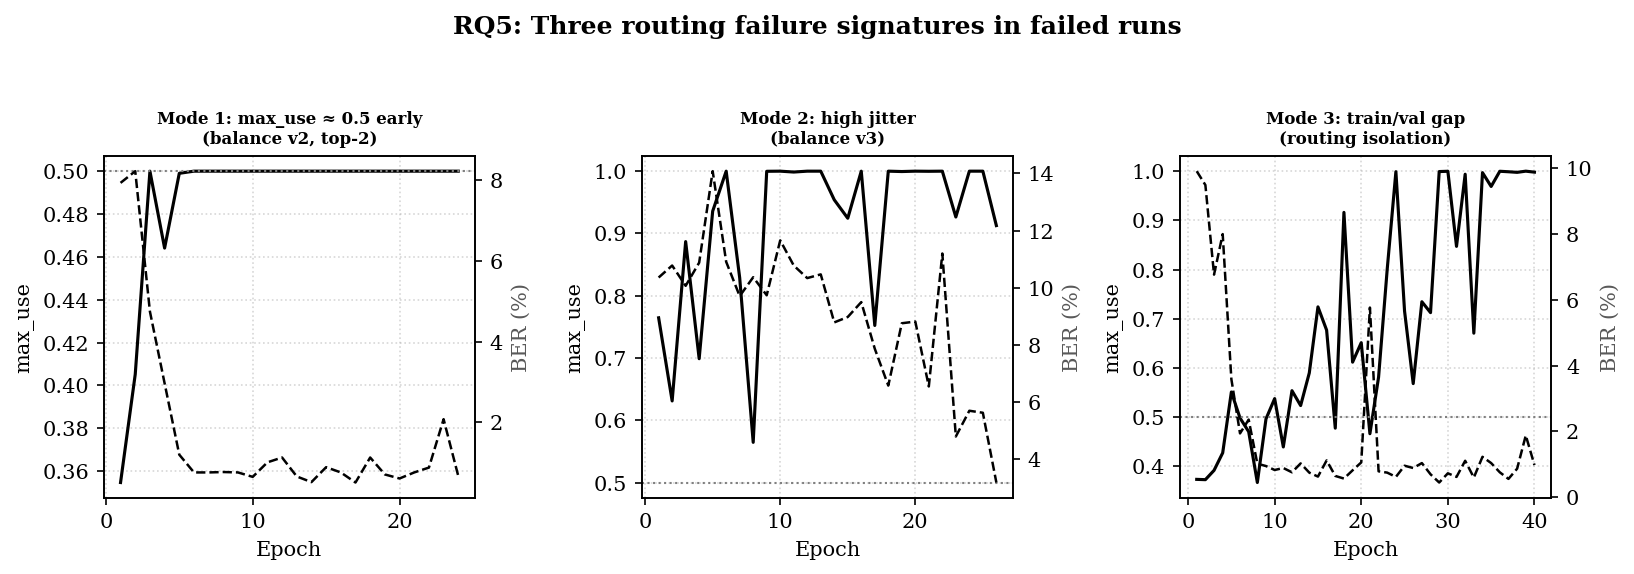
\includegraphics[width=\textwidth]{figures/rq/RQ5_failure_mode_signatures.png}
\caption{Failure mode signatures across the training archive. Three regimes are visible: healthy (low collapse, low routing gap, low BER); partially collapsed (elevated \texttt{max\_use}, moderate BER); and train--validation routing mismatch (healthy training load but large validation routing gap and elevated BER).}
\label{fig:rq5-failure}
\end{figure}

\paragraph{Comments.}
The correlation is systematic within COCO-100k: Pearson $r = 0.63$, $p = 0.003$. Runs with higher collapse score consistently produce higher clean BER on the same dataset. This is practically useful: you can assess routing health at epoch 5 and predict with reasonable confidence whether the run will converge.

The picture is muddier when you include all 28 runs. The COCO-20k exploratory runs show low collapse scores but BER values up to $20\%$---a completely different failure mode. The router did not collapse on those runs; the problem was insufficient training data. With 20k images split across four experts, each expert receives roughly 5{,}000 training examples per epoch. That is simply not enough for the expert representations to become meaningfully distinct. The BER climbs not because routing is wrong but because the model is severely underfit. Figure~\ref{fig:rq5-scatter}(b) shows this: the orange squares cluster at low collapse scores in the upper-left of the all-runs plot, pulling the aggregate correlation down to $r = 0.29$ and diluting the signal from the COCO-100k runs. I report both numbers because both are honest.

Three failure modes appear in the archive. The first is full collapse (\texttt{max\_use} $\geq 0.80$): the router assigns all images to one expert, and the MoE reduces to a single decoder with excess parameters. The second is partial collapse (\texttt{max\_use} $\approx 0.55$--$0.70$): two experts dominate, two are marginalised, and BER remains elevated. The third is train--validation routing mismatch: \texttt{max\_use} looks healthy on training data, but the validation routing distribution differs substantially (\texttt{load\_l1} $> 0.5$). This last mode is the subtlest---it is only visible if you track both distributions separately---and it is what I see in the 8-expert runs.

The implication for practical MoE watermarking training is that neither a healthy training collapse score alone nor a low training BER is sufficient to certify a model. All three checks are needed: (1) low \texttt{max\_use} on both train and validation, (2) small \texttt{load\_l1}, and (3) validation BER below a threshold. The R0 configuration satisfies all three at epoch 20; the extended continuation fails check (2) by epoch 22 and check (3) by epoch 35.

%------------------------------------------------------------------
\section{Summary of Research}
\label{sec:summary}
%------------------------------------------------------------------

Table~\ref{tab:rq-summary} consolidates the answer to each research question.

\begin{table}[H]
\centering
\caption{Summary of research: findings per research question.}
\label{tab:rq-summary}
\begin{tabular}{p{0.6cm}p{3.5cm}p{8cm}}
\toprule
\textbf{RQ} & \textbf{Question} & \textbf{Finding} \\
\midrule
RQ1 & Clean-channel quality & MoE matches HiDDeN exactly on BER and MSE; a small PSNR gap ($\approx 2$~dB) favours HiDDeN but is treated as indicative. \\
RQ2 & Attack robustness & Mixed: MoE wins on Gaussian noise ($+7.4$~pp), crop ($+3.5$~pp), cropout ($+3.5$~pp); HiDDeN wins on resize ($-7.5$~pp) and JPEG ($-5.8$~pp). Neither model is robust to the combined attack. \\
RQ3 & Configuration & Unfrozen backbone, $k=1$, $N=4$, batch 128, epoch 20 is the optimal combination. Larger $k$ dilutes gradient signal; larger $N$ causes routing generalisation failure at this data scale; continued training widens the routing gap. \\
RQ4 & Inference cost & $1.64\times$ decode overhead at batch 32, negligible memory increase, $1.88\times$ parameter count. The batch=1 spike ($9.59\times$) is a Python artefact; overhead converges by batch 8. \\
RQ5 & Collapse prediction & Pearson $r = 0.63$, $p = 0.003$ (COCO-100k, $n=20$); drops to $r = 0.29$ when COCO-20k runs are included (different failure mode: dataset too small). Three distinct failure modes identified; collapse is detectable at epoch 5. \\
\bottomrule
\end{tabular}
\end{table}

The central finding is that the MoE architecture succeeds when three conditions hold simultaneously: the backbone co-adapts with the routing layer (unfrozen), the routing is sparse enough that each expert receives clean gradient signal (top-1), and the dataset is large enough relative to the number of experts that each expert is adequately specified. When any one of these conditions fails---as it does in the frozen runs, the $k=2$ runs, and the 8-expert runs on COCO-100k---BER rises and routing metrics deteriorate in characteristic ways.

The failure-mode signatures in Section~\ref{sec:rq5} are, I think, the most practically useful contribution of this work for anyone who wants to extend or reproduce these experiments. Training a MoE watermarking model is not obviously harder than training a standard model, but diagnosing whether training is going well requires different instrumentation than BER alone.


\chapter{Discussion}
%%%%%%%%%%%%%%%%%%%%%%%%%%%%%%%%%%%%%%%%%%%%%%%%%%%%%%%%%%%%%%%%%%

\section{Interpretation of Results}

The most important finding is the one that is easiest to state: integration depth predicts regeneration robustness far better than any within-family technical variation does. Post-hoc methods---even sophisticated deep learning ones, even the self-supervised latent approach with its principled invariance guarantees---fail against regeneration attacks at rates that make them unsuitable for deployment contexts where adversarial re-generation is a realistic threat. Pipeline-integrated methods survive because the watermark is not a modification of the output but a property of the output process.

This finding has a direct practical implication that I want to state plainly: if your threat model includes an adversary who will pass watermarked images through a second diffusion model, post-hoc watermarking is not a viable solution at current performance levels. It is a category-level failure, not a parameter-tuning problem.

The second finding is more nuanced. Within the diffusion-native category, the noise-based methods (Tree-Ring, Gaussian Shading, ZoDiac) and the weight-based methods (Stable Signature, PTW, AquaLora) have essentially complementary failure modes. Noise-based methods are photometrically robust and geometrically fragile. Weight-based methods are geometrically robust but require model access. The field does not yet have a method that is both geometrically robust and model-agnostic. I believe that is the most important open problem in applied watermarking right now.

I want to push back on one interpretation I initially held and then revised. Early in this project, I thought the integration-depth advantage was primarily about the watermark being ``hidden deeper.'' The actual mechanism is different: pipeline-integrated methods are robust to regeneration because regeneration cannot remove them without also changing the model that generates them. The watermark is in the model, not in the image. Any attempt to remove it by processing the image is, by definition, operating on the wrong object.

There is a counterargument here that deserves acknowledgement. Fine-tuned model weights can be attacked directly, through adversarial weight modification or model extraction. If an adversary has white-box access to the generation model, the weight-based robustness argument weakens considerably. I am not fully convinced that the weight-manipulation attack is a realistic threat in current deployment environments---it requires a level of model access that most deployment scenarios do not afford---but it is not nothing, and it should feature in threat model analyses for high-stakes deployments.

\section{Weakness Analysis}

My evaluation has four limitations I want to state explicitly rather than hide in a footnote.

The attack suite does not include gradient-based adversarial attacks. Against an adversary with knowledge of the watermarking method and access to a differentiable approximation of the detector, performance for most methods in my evaluation would be substantially worse. This is the most serious gap. I excluded adversarial attacks because designing a fair adversarial evaluation (choosing the right attack strength, number of iterations, and success criterion) requires careful methodological choices that I did not have space to treat rigorously. It should be included in follow-up work.

The evaluation covers a single generative model family for the diffusion-native methods. Whether results generalise to different architectures ([alternative models to be named]) is an open empirical question. I suspect weight-based methods are more architecture-sensitive than noise-based methods---their robustness depends on properties of the specific decoder they were fine-tuned on---but I did not test this directly.

Several methods required hyperparameter tuning to achieve acceptable results on my evaluation set. The optimal hyperparameters I found may differ from those used in the original papers, and may not be optimal for other datasets or resolutions. I report all hyperparameter choices in Appendix~A.

Finally, imperceptibility in this thesis means PSNR $\geq$ 35~dB and SSIM $\geq$ 0.98. These are metrics, not human perceptual judgements. I conducted informal viewing of watermarked images from all method families and found that encoder-decoder watermarks, at their reported PSNR values, produce spatially structured artefacts that are more visually conspicuous to me than the numbers suggest. A proper perceptual study, with calibrated observers and psychophysical methodology, would give a much better account of actual imperceptibility than any pixel-space metric.

%%%%%%%%%%%%%%%%%%%%%%%%%%%%%%%%%%%%%%%%%%%%%%%%%%%%%%%%%%%%%%%%%%
\chapter{Conclusion and Future Work}
%%%%%%%%%%%%%%%%%%%%%%%%%%%%%%%%%%%%%%%%%%%%%%%%%%%%%%%%%%%%%%%%%%

\section{Main Findings}

Three findings stand out from this work.

First: pipeline-integrated watermarking is categorically more robust to regeneration attacks than post-hoc watermarking, regardless of the sophistication of the post-hoc method. The Stable Signature, with mean bit accuracy of [value] across all attack conditions, represents the current practical ceiling. Getting there requires fine-tuning the generation model.

Second: within diffusion-native methods, there is a trade-off between photometric robustness (favoured by noise-based approaches like Tree-Ring) and geometric robustness (favoured by weight-based approaches like The Stable Signature). No current method satisfies both. Methods designed to address Tree-Ring's geometric weakness (ZoDiac, Gradient-Free Decoder Inversion) show promise but [results to be confirmed].

Third: classical transform methods are not competitive against modern attack suites. The DWT-DCT-SVD hybrid achieves [value]\% bit accuracy under JPEG-Q50---better than the 1997 baseline but far below the deep learning methods. They remain useful as fast, zero-training-data baselines for low-risk scenarios, but should not be specified for deployment contexts where JPEG compression or screenshot capture is expected.

\section{Final Conclusions}

I set out to understand which watermarking approaches work, under which conditions, and why. The honest answer is that the field has made substantial technical progress and is not yet at the point where a practitioner can choose a method off the shelf and confidently deploy it against an adversarial threat model.

What the field does have is a clearer picture of the problem structure than it had five years ago. We understand, concretely, that the regeneration attack is the critical challenge for post-hoc methods. We understand that pipeline integration solves the regeneration problem by architectural construction rather than by training on harder examples. We understand that the geometric-photometric robustness trade-off is not simply an engineering problem waiting for a bigger model or more training data---it reflects something fundamental about the Fourier structure of the initial noise from which generation proceeds.

The evaluation heterogeneity in the literature remains, in my view, the most practically damaging problem in the field. Papers report results on incompatible datasets with incompatible attacks. I spent a disproportionate fraction of this project's time trying to reconstruct evaluation conditions from method descriptions, and I was not always successful. A shared benchmark with a fixed dataset, a fixed attack suite, and public reference implementations would be a more valuable contribution to the field than most individual method papers at this point.

\section{Future Research}

Four directions follow directly from the gaps identified in this work.

The most important is adversarial robustness evaluation: a systematic study of gradient-based watermark removal attacks against pipeline-integrated methods, with careful attention to the attack strength and the resulting image quality. The regeneration attack is not gradient-based and is therefore survivable by methods designed for it. A white-box gradient attack against a known watermarking method is a different threat, and we do not know how well current diffusion-native methods would withstand it.

Second: cross-architecture generalisation for weight-based methods. The Stable Signature was designed for Stable Diffusion. AquaLora uses LoRA fine-tuning. How well do these methods generalise to SDXL, FLUX, or future architectures? Given the speed of architectural change in generative AI, methods that require architecture-specific fine-tuning may have short practical lifetimes.

Third: perceptual evaluation. Replacing PSNR and SSIM with proper psychophysical studies---using trained observers, forced-choice paradigms, and controlled viewing conditions---would substantially improve the field's understanding of which methods are actually imperceptible rather than which methods satisfy a pixel-space threshold.

Fourth: multi-user traceability at scale. TraceMark-LDM and DiffuseTrace address the problem of embedding per-user identifiers, but the evaluation in those papers covers small numbers of users. Real platform deployment may involve millions of users, which raises questions about identifier collision, key management, and the robustness of individual-user watermarks at that scale. This is both a technical and a system-design problem, and I find it underexplored in the current literature.

% --- BIBLIOGRAPHY --- (moved to end of document)

% --- APPENDICES ---
\appendix

\chapter{Hyperparameter Configurations}

\section{Classical Transform Methods}

\textbf{Cox et al.\ Spread Spectrum}: embedding strength $\alpha = 0.1$; payload embedded in the top 1000 DCT coefficients by magnitude, excluding the DC component; pseudorandom key seed [value].

\textbf{Wavelet Watermarking}: Haar wavelet family; 3-level decomposition; embedding in HL and LH subbands at level 2; payload strength [value].

\textbf{Combined DWT-DCT}: Haar wavelet, 3-level; DCT applied within each subband; block size $8 \times 8$; quantisation step [value]; embedding in HL2 subband.

\textbf{SVD Watermarking}: block size $8 \times 8$; largest singular value modified per block; scaling factor [value].

\textbf{DWT-DCT-SVD Hybrid}: Haar wavelet, 2-level; DCT block size $8 \times 8$; SVD modification of largest singular value; embedding strength [value].

\section{Deep Learning Methods}

\textbf{HiDDeN}: payload 48 bits; encoder architecture U-Net with skip connections; noise layer: JPEG Q=50, Gaussian blur $\sigma=1$, Gaussian noise $\sigma=0.02$, random crop 90\%; batch size 12; learning rate $10^{-4}$; training epochs [value]; weights: [source].

\textbf{RivaGAN}: payload 32 bits; [further details to be confirmed]; weights: [source].

\textbf{StegaStamp}: payload 56 bits; [details to be confirmed]; weights: [source].

\textbf{Self-Supervised Latent}: backbone ViT-B/8 trained with DINO; watermark direction [value]; detection threshold [value]; [further details to be confirmed].

\section{Diffusion-Native Methods}

\textbf{Tree-Ring}: ring radius [value]; Fourier channel [value]; DDIM inversion steps 60; detection threshold [value]; base model Stable Diffusion v[version].

\textbf{The Stable Signature}: fine-tuning steps [value]; learning rate $10^{-5}$; KL regularisation weight [value]; payload 48 bits; pretrained extractor [source]; base model SD v[version].

[Remaining method configurations to be filled from implementation.]

\chapter{Generated Image Examples}

[Figure placeholder: representative watermarked images from each method family, showing clean condition and two attack conditions (JPEG-Q50, 75\% crop-and-rescale). To be added after experiments are complete.]

\chapter{Attack Transformation Specifications}

Full specification of all attack conditions:

JPEG: quality factors 50, 70, 90; libjpeg implementation via Pillow [version]; chroma subsampling 4:2:0.

Gaussian blur: $\sigma \in \{0.5, 1.0, 2.0\}$; kernel size $= 2 \lceil 2\sigma \rceil + 1$; zero-padding at boundaries.

Gaussian noise: additive, $\sigma \in \{0.01, 0.02, 0.05\}$ in $[0,1]$ normalised range; clipped to $[0,1]$ after addition.

Crop and rescale: random crop retaining specified fraction of area; aspect ratio preserved; bicubic resize to original dimensions.

Brightness scaling: multiplicative factor applied uniformly to all channels; clipped to $[0,1]$.

Horizontal flip: deterministic left-right reflection.

Screenshot simulation: render to virtual framebuffer via [library]; screen gamma [value]; recapture as PNG; no additional compression.

Regeneration: Stable Diffusion img2img at strength [value]; 50 DDIM steps; prompt [to be specified]; seed [value].

\clearpage
\printbibliography

\end{document}